\documentclass[11pt,letterpaper]{article}

% Compile from the folder containing this file.
% This path works in template/ and in sibling course folders.
% Shared formatting for course notes. Loaded by each course's main.tex.
\usepackage[T1]{fontenc}
\usepackage[utf8]{inputenc}
\usepackage{lmodern}
\linespread{1.15}
\usepackage[margin=1in]{geometry}
\usepackage{amsmath,amssymb,amsthm}
\usepackage{mathtools}
\usepackage{graphicx}
\usepackage{booktabs}
\usepackage{enumitem}
\usepackage{xcolor}
\usepackage{hyperref}
\usepackage{tikz}
\usetikzlibrary{decorations.pathreplacing,positioning}
\usepackage{xparse}
\usepackage{etoolbox}

\hypersetup{colorlinks=true,linkcolor=blue!50!black,urlcolor=blue!50!black}
\setlength{\parindent}{0pt}
\setlength{\parskip}{0.5em}
\setlist{nosep}

% Unnumbered section headings: entries show as "Week 1", not "1 Week 1",
% both in the body and in the table of contents.
\setcounter{secnumdepth}{0}

% Each \section (i.e. each week's entry) starts on its own new page. The
% \newpage that used to follow \tableofcontents in each course's main.tex
% is redundant now and has been removed, so week 1 isn't pushed to a blank
% page by this.
\pretocmd{\section}{\newpage}{}{\errmessage{Failed to patch \string\section}}

% Tracks whether \section was the most recent sectioning/lecture command,
% so a \newlecture immediately following a \section (the usual "week's
% first lecture" case) doesn't also throw in its own \newpage, which would
% otherwise leave a blank page between the two. Set true by \section, and
% cleared by \newlecture whether or not it was true, so it only fires for
% a \newlecture that directly follows a \section (nothing else in between).
\newbool{newlecture@justsection}
\pretocmd{\section}{\booltrue{newlecture@justsection}}{}{\errmessage{Failed to patch \string\section}}

% Custom head format: bold, unparenthesized title, with a \quad gap after
% the number (e.g. "Theorem 3.2  Distribution" instead of "Theorem 3.2
% (Distribution)."), reusing amsthm's usual spacing/punctuation otherwise.
% When a title is given, the body text starts on its own new line below the
% head instead of running inline after it; untitled (auto-numbered-only)
% instances stay inline as usual. Body text is upright (not italic) for all
% six environments. Two variants share this head format but differ in
% end-of-head punctuation: theorem/lemma/proposition/exercise keep a
% trailing period, definition/example drop it (no period after the title).
\makeatletter
\newcommand{\thmpunct}{.}
\newtheoremstyle{boldhead}{}{}{\normalfont}{}{\bfseries}{\thmpunct}{5pt plus 1pt minus 1pt}%
    {\thmname{#1}\thmnumber{\@ifnotempty{#1}{ }#2}\thmnote{\@ifnotempty{#3}{\quad#3}}%
     \@ifnotempty{#3}{\def\thmheadnl{\newline}\thm@headsep\z@skip}{}}
\newtheoremstyle{boldheadnp}{}{}{\normalfont}{}{\bfseries}{}{5pt plus 1pt minus 1pt}%
    {\thmname{#1}\thmnumber{\@ifnotempty{#1}{ }#2}\thmnote{\@ifnotempty{#3}{\quad#3}}%
     \@ifnotempty{#3}{\def\thmheadnl{\newline}\thm@headsep\z@skip}{}}
\makeatother

\theoremstyle{boldhead}
\newtheorem{theorem}{Theorem}
\newtheorem{lemma}[theorem]{Lemma}
\newtheorem{proposition}[theorem]{Proposition}
\newtheorem{corollary}[theorem]{Corollary}
\newtheorem{exercise}[theorem]{Exercise}
\theoremstyle{boldheadnp}
\newtheorem{definition}[theorem]{Def.}
\newtheorem{example}[theorem]{Example}
\theoremstyle{remark}
\newtheorem*{remark}{Remark}

% \begin{theorem}[Title][2.7]: both optional arguments are new on top of
% the environments' usual single bracket. The first argument still behaves
% exactly like plain amsthm's optional title (existing notes using
% \begin{example}[Some Name] etc. are unaffected). The second argument, if
% given, overrides the displayed number (e.g. to match a textbook's own
% numbering) instead of the shared theorem counter's automatic value; the
% counter itself still advances normally, so later auto-numbered
% environments are unaffected too.
\newcommand{\addtitleandnumber}[1]{%
    \csletcs{#1orig}{#1}%
    \csletcs{end#1orig}{end#1}%
    \RenewDocumentEnvironment{#1}{o o}{%
        \IfValueT{##2}{\ifblank{##2}{}{\renewcommand{\thetheorem}{##2}}}%
        \IfValueTF{##1}{\ifblank{##1}{\csname#1orig\endcsname}{\csname#1orig\endcsname[##1]}}{\csname#1orig\endcsname}%
    }{\csname end#1orig\endcsname}%
}
\addtitleandnumber{theorem}
\addtitleandnumber{lemma}
\addtitleandnumber{proposition}
\addtitleandnumber{corollary}
\addtitleandnumber{definition}
\addtitleandnumber{example}
\addtitleandnumber{exercise}

% Common mathematical notation.
\newcommand{\R}{\mathbb{R}}
\newcommand{\N}{\mathbb{N}}
\newcommand{\Z}{\mathbb{Z}}
\newcommand{\E}{\mathbb{E}}
\newcommand{\Prob}{\mathbb{P}}
\DeclareMathOperator{\Var}{Var}
\DeclareMathOperator{\Cov}{Cov}

% \newlecture[title][date]: bold, centered marker for the start of a new
% lecture. Both arguments are optional. Numbering runs continuously across
% the whole document (i.e. across all weeks' entries, not reset per
% \section), so the Nth \newlecture in the course is always "Lecture N".
% Each lecture starts on its own new page, except when it directly follows
% a \section heading (which already started a new page of its own), so the
% two stay together instead of leaving a blank page in between.
\newcounter{lecture}
\renewcommand{\thelecture}{\arabic{lecture}}
% Set \lecturetoctrue in a course's main.tex to list each lecture as a
% top-level table-of-contents entry ("Lecture N: title", or the date when
% untitled), with \subsection headings nested beneath it.
\newif\iflecturetoc
\NewDocumentCommand{\newlecture}{o o}{%
    \stepcounter{lecture}%
    \ifbool{newlecture@justsection}{}{\newpage}%
    \boolfalse{newlecture@justsection}%
    \iflecturetoc
        \phantomsection
        \addcontentsline{toc}{section}{Lecture \thelecture\IfValueTF{#1}{\ifblank{#1}{\IfValueT{#2}{\ifblank{#2}{}{ (#2)}}}{: #1}}{\IfValueT{#2}{\ifblank{#2}{}{ (#2)}}}}%
    \fi
    \par\vspace{1em}
    \begin{center}
        \textbf{\Large Lecture \thelecture\IfValueT{#1}{: #1}}\\[2pt]
        \IfValueT{#2}{\normalsize #2}
    \end{center}
    \vspace{0.5em}%
}

% Handwritten-note-style helpers: red definition labels, blue margin
% annotations, yellow highlights, underlined mini-headers.
\newcommand{\deflabel}[2]{\par\noindent{\color{red!70!black}\textbf{Def #1}}\quad\textbf{#2}\par\nobreak}
\newcommand{\exlabel}[2]{\par\noindent\textbf{Example #1}\quad\textbf{#2}\par\nobreak}
\newcommand{\heading}[1]{\par\noindent{\color{red!70!black}\textbf{#1}}\par}
\newcommand{\header}[1]{\par\vspace{0.5em}\noindent\textbf{#1}\par\vspace{-0.2em}}
\newcommand{\aside}[1]{\ifmmode{\color{blue!55!black}\text{\itshape #1}}\else{\color{blue!55!black}\itshape #1}\fi}
\newcommand{\hly}[1]{\colorbox{yellow!55}{$#1$}}
\newcommand{\hlt}[1]{\colorbox{yellow!55}{#1}}
% \boldmath makes any math the argument switches into (e.g. \rb{$r$}) use
% the bold math version automatically, so callers don't need to manually
% wrap math content in \boldsymbol{}.
\newcommand{\rb}[1]{{\color{red!70!black}\boldmath\textbf{#1}}}
\renewcommand{\b}[1]{\textbf{#1}}
\definecolor{navy}{RGB}{0,32,96}
\newcommand{\dbb}[1]{{\color{navy}\textbf{#1}}}
\newcommand{\db}[1]{{\color{navy}#1}}

% Wider padding inside \boxed{} equations (default \fboxsep is 3pt).
% Scoped to \boxed only, so \colorbox highlights (e.g. \hly) are unaffected.
\let\oldboxed\boxed
\renewcommand{\boxed}[1]{{\setlength{\fboxsep}{10pt}\oldboxed{#1}}}

\usepackage{framed}
\usepackage{soul} % \ul: underline that can break across lines
\usepackage{cancel} % \cancel: strike out terms that cancel
\renewcommand{\CancelColor}{\color{red!70!black}}

% Definitions in this course aren't numbered.
\theoremstyle{boldheadnp}
\let\definition\relax
\let\enddefinition\relax
\newtheorem*{definition}{Def.}

% Examples in this course aren't numbered, are labeled "Ex.", and are boxed.
\theoremstyle{boldheadnp}
\let\example\relax
\let\endexample\relax
\newtheorem*{exampleinner}{Ex.}
\newenvironment{example}
    {\begin{framed}\vspace{-0.5em}\begin{exampleinner}}
    {\end{exampleinner}\end{framed}}

% Red-bordered box for key takeaways (like the boxed statements on the slides).
\newcommand{\keypoint}[1]{\par\begin{center}{\setlength{\fboxsep}{6pt}\setlength{\fboxrule}{0.8pt}\fcolorbox{red!70!black}{white}{\parbox{0.9\linewidth}{\centering #1}}}\end{center}}

% Tight rounded box to circle a term inside an equation (e.g. a factor being multiplied in).
\newcommand{\emphbox}[1]{\tikz[baseline=(X.base)]\node[draw=red!70!black, thick, rounded corners=3pt, inner sep=1.5pt] (X) {$\displaystyle #1$};}

% Replace these details for each course.
\newcommand{\coursecode}{MIE375}
\newcommand{\coursename}{Financial Engineering}
\newcommand{\term}{Fall 2026}
\newcommand{\studentname}{Bonnie Zhuang}

\title{\coursecode{} --- \coursename\\[0.5em]\large Course Notes}
\author{\studentname}
\date{\term}

\lecturetoctrue

\begin{document}
\maketitle
\tableofcontents

% Add one input per lecture, in the order you want them to appear.
% !TeX root = ../main.tex

\newlecture[Introduction/Syllabus][September 14, 2026]

\header{Principal and Interest}
\begin{definition}
    Principal: Amount invested

    Interest: "Rent" paid on investment
\end{definition}

In general, for
\begin{itemize}
    \item $A$: Principal
    \item $r$: interest rate per period
    \item $V$: Value received.
\end{itemize}
After 1 period, $V=A(1+r) = A + Ar$ is received, where $Ar$ is the interest earned on the principal for one period.

\begin{example}
    Invest \$1 for 1 year at 8\%: after 1 year you receive
    \[\$1.08 = \underbrace{\$1.00}_{\text{principal}} + \underbrace{\$0.08}_{\text{interest}}\]
\end{example}

Interest over multiple periods depend on the compounding rules:
\begin{enumerate}
    \item \rb{Simple}: Money grows linearly, receiving $V=A(1+nr)$ over $n$ periods.
    \item \rb{Compound}: Money grows geometrically, receiving $V=A(1+r)^n$ over $n$ periods.
\end{enumerate}

The Rule of 72: Money invested at $r\%$ per year doubles in approximately $72/r$ years.

\begin{example}
    \textit{Simple:} \$5000 borrowed for 5 years at 10\% per year simple interest is owed
    \[V = A(1+rn) = 5000(1+0.1\cdot 5) = \$7500\]
    \textit{Compound:} \$100 deposited at 7\% compounded yearly for 10 years grows to
    \[V = A(1+r)^n = 100(1+0.07)^{10} = \$196.72\]
\end{example}
Simple interest is not used often in practice.


\begin{definition}
    \rb{Nominal Interest Rate}: annual quote, compounding interest is in fractions corresponding to the compounding period.
    \\For $m$ periods per year for $k$ periods, $V=A(1+\frac{r}{m})^k$
\end{definition}

\begin{example}
    Invest \$10 at 8\% compounded quarterly for 3 quarters:
    \[V = 10\left(1+\frac{0.08}{4}\right)^3 = \$10.61\]
\end{example}

\begin{definition}
    \rb{Continuous Compound Interest}: when the compounding period becomes arbitrarily small, the value approaches $e^{rt}$.
\end{definition}
After 1 year with $m$ periods: $(1+\frac{r}{m})^m$, and $\lim_{m\to\infty}(1+\frac{r}{m})^m = e^r$. More generally, in $t$ years there are $k = tm$ periods, so $(1+\frac{r}{m})^{tm} \to e^{rt}$.

\begin{example}
    $A = \$100$, $r = 9\%$ compounded continuously. After 1.5 years:
    \[V = 100e^{(0.09)(1.5)} = \$114.45\]
\end{example}

\header{Compound Interest Summary}
For $r$ the nominal interest rate quoted:
\[\boxed{\begin{gathered}
    \text{Yearly for $k$ years:} \quad (1+r)^k\\
    \text{$m$ periods per year for $k$ periods:} \quad \left(1+\frac{r}{m}\right)^k\\
    \text{Continuously for time $t$:} \quad e^{rt}
\end{gathered}}\]

\begin{definition}
    \rb{Effective Rate}: interest rates are usually quoted as nominal rates, but what you pay depends on the number of compounding periods. The equivalent rate with a \textit{single} compounding period over the time interval of interest is the effective rate.
\end{definition}

Relationship between Nominal and Effective Rate (with $m$ compounding periods per year, so the rate per compounding period is $r = r_{nom}/m$):
\[1+ r_{eff} = (1+ \frac{r_{nom}}{m})^m \quad \Rightarrow \quad \boxed{r_{eff} = (1+ \frac{r_{nom}}{m})^m - 1}\]
\[\text{1 + Simple One-year Rate = the Explicit Compound}\]

\begin{example}
    Effective yearly rate of 8\% compounded quarterly:
    \[r_{eff} = \left(1+\frac{0.08}{4}\right)^4 - 1 = 8.24\%\]
\end{example}

\begin{definition}
    \rb{APR} (Annual Percentage Rate): the \textit{nominal} annual rate of interest including all fees and charges.
    \\\rb{APY} (Annual Percentage Yield): the \textit{effective} annual rate of interest including all fees and charges.
\end{definition}
Both are required by the Truth in Lending Act (1968), and can be used to compare loans with different terms.

\begin{example}[Credit Card]
    A credit card statement lists \textit{daily} periodic rates of 0.02986\% (purchases) and 0.05477\% (advances).
    \begin{center}
    \begin{tabular}{lcc}
        \toprule
        & Nominal (APR) & Effective\\
        \midrule
        Purchases & $(0.02986\%)(365) = 10.900\%$ & $(1.0002986)^{365} - 1 = 11.514\%$\\
        Advances & $(0.05477\%)(365) = 19.990\%$ & $(1.0005477)^{365} - 1 = 22.121\%$\\
        \bottomrule
    \end{tabular}
    \end{center}
    The statement's ``annual percentage rate'' is the nominal rate; the rate you actually pay is the higher effective rate.
\end{example}

\header{Practice Problems}
\begin{example}
    Yearly effective rate corresponding to:
    \begin{enumerate}[label=(\alph*)]
        \item 8\% compounded monthly: $\left(1+\frac{0.08}{12}\right)^{12} - 1 = 8.30\%$
        \item 5\% compounded semi-annually: $\left(1+\frac{0.05}{2}\right)^{2} - 1 = 5.06\%$
        \item 10\% compounded continuously: $e^{0.10} - 1 = 10.52\%$
    \end{enumerate}
\end{example}

\begin{example}
    Convert by matching effective rates:
    \begin{enumerate}[label=(\alph*)]
        \item 3\% compounded quarterly to the nominal rate compounded monthly:
        \[\left(1+\frac{r}{12}\right)^{12} = \left(1+\frac{0.03}{4}\right)^{4} \quad \Rightarrow \quad r = 12\left[(1.0075)^{1/3} - 1\right] = 2.99\%\]
        \item 6\% compounded semi-annually to the nominal rate compounded continuously:
        \[e^{r} = \left(1+\frac{0.06}{2}\right)^{2} \quad \Rightarrow \quad r = 2\ln(1.03) = 5.91\%\]
    \end{enumerate}
\end{example}

\begin{example}
    Which rate would you choose? Compare the effective rates:
    \begin{center}
    \begin{tabular}{lc}
        \toprule
        Quoted rate & Effective yearly rate\\
        \midrule
        (a) 10\% compounded continuously & 10.52\%\\
        (b) 10.3\% compounded monthly & 10.80\%\\
        (c) 10.5\% compounded quarterly & 10.92\%\\
        (d) 10.6\% compounded yearly & 10.60\%\\
        \bottomrule
    \end{tabular}
    \end{center}
    As an investor, choose (c) since it has the highest effective rate (as a borrower, choose (a)).
\end{example}

\header{Commonly Referred to Interest Rates}
\begin{itemize}
    \item \b{Discount Rate}: the rate at which member banks may borrow short term funds directly from a federal reserve bank.
    \item \b{Federal Funds Rate}: the rate that banks charge each other for the use of federal funds.
    \item \b{Prime Rate}: the interest rate that commercial banks charge their most creditworthy borrowers.
    \item \b{LIBOR} (London Inter-Bank Offer Rate): the interest rate that banks charge each other for loans (usually in Eurodollars).
\end{itemize}

% !TeX root = ../main.tex

\newlecture[Present Value and Internal Rate of Return][Sep 17, 2026]
Present value: comparing cash flows that occur at different times, while interest rates tells how to move cash flows in time. Use interest rates to move all cash flows to the same time, so they become easy to compare.

\b{Ideal Bank}: applies the same rate of interest to deposits and loans, and has no transaction costs (real banks have higher rates for loans...).
Used for two ways:
\begin{itemize}
    \item \rb{Compounding}: when cash flow is moved \b{forward}, \dbb{multiplied} by $(1+r)$ each period.
    \item \rb{Discounting}: when cash flow is moved \b{backward}, \dbb{divided} by $(1+r)$ each period.
\end{itemize}

\begin{center}
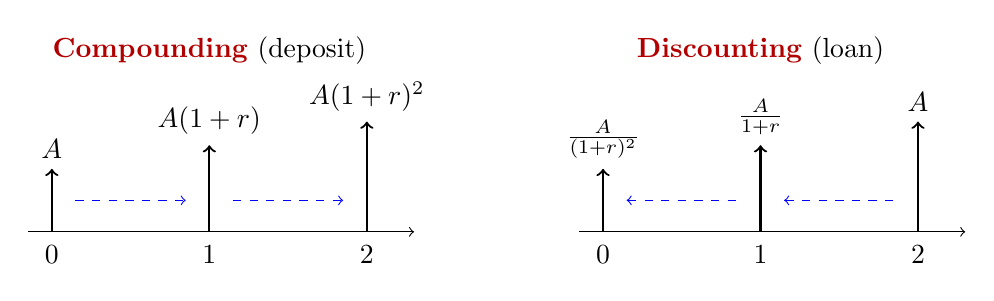
\begin{tikzpicture}
    \node at (2,2.3) {\rb{Compounding} (deposit)};
    \draw[->] (-0.3,0) -- (4.6,0);
    \foreach \x in {0,1,2} { \node[below] at (2*\x,-0.05) {$\x$}; }
    \draw[->, thick] (0,0) -- (0,0.8) node[above] {$A$};
    \draw[->, thick] (2,0) -- (2,1.1) node[above] {$A(1+r)$};
    \draw[->, thick] (4,0) -- (4,1.4) node[above] {$A(1+r)^2$};
    \draw[->, blue, dashed] (0.3,0.4) -- (1.7,0.4);
    \draw[->, blue, dashed] (2.3,0.4) -- (3.7,0.4);
    \begin{scope}[xshift=7cm]
        \node at (2,2.3) {\rb{Discounting} (loan)};
        \draw[->] (-0.3,0) -- (4.6,0);
        \foreach \x in {0,1,2} { \node[below] at (2*\x,-0.05) {$\x$}; }
        \draw[->, thick] (0,0) -- (0,0.8) node[above] {$\frac{A}{(1+r)^2}$};
        \draw[->, thick] (2,0) -- (2,1.1) node[above] {$\frac{A}{1+r}$};
        \draw[->, thick] (4,0) -- (4,1.4) node[above] {$A$};
        \draw[<-, blue, dashed] (0.3,0.4) -- (1.7,0.4);
        \draw[<-, blue, dashed] (2.3,0.4) -- (3.7,0.4);
    \end{scope}
\end{tikzpicture}
\end{center}

\header{The Comparison Principle}
The ideal bank brings cash flow stream to the same time, then is compared.
\begin{itemize}
    \item When all cash flows are moved to \textit{present time}, it is called \rb{present value}.
    \item When all cash flows are moved to the \textit{time of the final cash flow}, it is called \rb{future value}.
\end{itemize}

\begin{center}
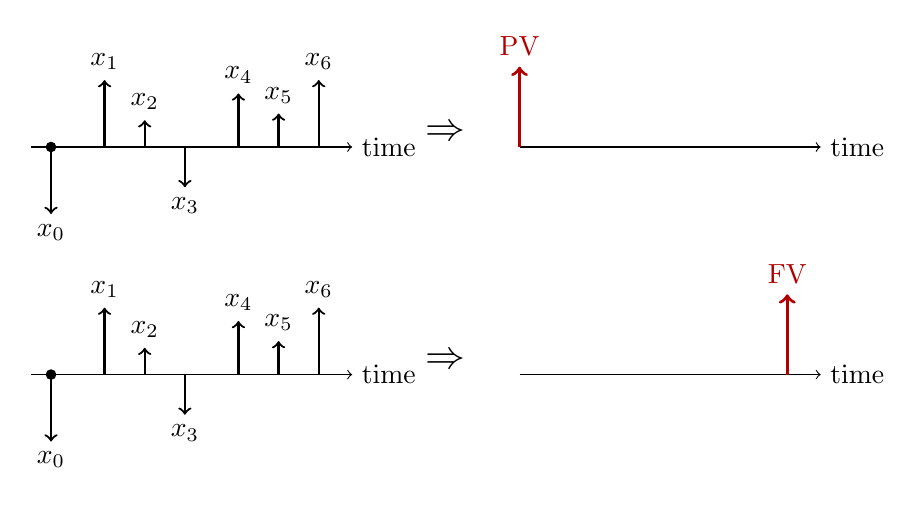
\begin{tikzpicture}[scale=0.85]
    \foreach \row/\lab/\px in {0/PV/0, -3.4/FV/4} {
        \begin{scope}[yshift=\row cm]
            \draw[->] (-0.3,0) -- (4.5,0) node[right] {time};
            \filldraw (0,0) circle (2pt);
            \draw[->, thick] (0,0) -- (0,-1) node[below] {$x_0$};
            \draw[->, thick] (0.8,0) -- (0.8,1) node[above] {$x_1$};
            \draw[->, thick] (1.4,0) -- (1.4,0.4) node[above] {$x_2$};
            \draw[->, thick] (2.0,0) -- (2.0,-0.6) node[below] {$x_3$};
            \draw[->, thick] (2.8,0) -- (2.8,0.8) node[above] {$x_4$};
            \draw[->, thick] (3.4,0) -- (3.4,0.5) node[above] {$x_5$};
            \draw[->, thick] (4.0,0) -- (4.0,1) node[above] {$x_6$};
            \node at (5.9,0.2) {\Large$\Rightarrow$};
            \draw[->] (7,0) -- (11.5,0) node[right] {time};
            \draw[->, very thick, red!70!black] (7+\px,0) -- (7+\px,1.2) node[above] {\lab};
        \end{scope}
    }
\end{tikzpicture}
\end{center}

\begin{example}
    Cash flow stream $(-2,1,1,1)$ at $r = 10\%$ (yearly compounding, but any compounding convention works):
    \begin{align*}
        FV &= -2(1.1)^3 + 1(1.1)^2 + 1(1.1) + 1 = 0.648\\
        PV &= -2 + \frac{1}{1.1} + \frac{1}{(1.1)^2} + \frac{1}{(1.1)^3} = 0.487
    \end{align*}
    Check: $PV = FV/(1.1)^3 = 0.648/(1.1)^3 = 0.487$
\end{example}

\header{General Formula for Present Value}
\begin{center}
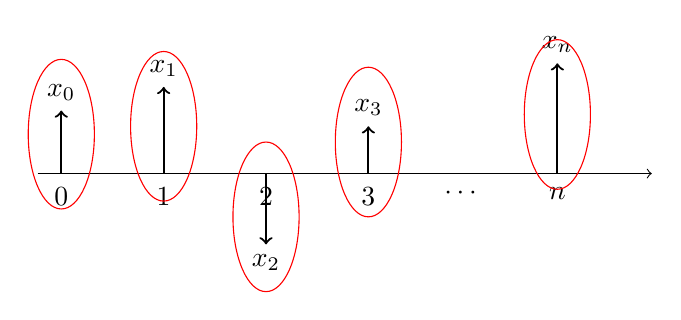
\begin{tikzpicture}
    \draw[->] (-0.3,0) -- (7.5,0);
    \foreach \x/\l in {0/0,1.3/1,2.6/2,3.9/3,6.3/n} { \node[below] at (\x,-0.05) {$\l$}; }
    \node[below] at (5.1,-0.05) {$\cdots$};
    \draw[->, thick] (0,0) -- (0,0.8) node[above] {$x_0$};
    \draw[->, thick] (1.3,0) -- (1.3,1.1) node[above] {$x_1$};
    \draw[->, thick] (2.6,0) -- (2.6,-0.9) node[below] {$x_2$};
    \draw[->, thick] (3.9,0) -- (3.9,0.6) node[above] {$x_3$};
    \draw[->, thick] (6.3,0) -- (6.3,1.4) node[above] {$x_n$};
    \foreach \x/\y in {0/0.5,1.3/0.6,3.9/0.4,6.3/0.75} { \draw[red] (\x,\y) ellipse (0.42 and 0.95); }
    \draw[red] (2.6,-0.55) ellipse (0.42 and 0.95);
\end{tikzpicture}
\end{center}
Each cash flow (circled) is discounted separately, then all are summed. Let $x = (x_0, x_1, x_2, \dots, x_n)$
\begin{align*}
    PV(x) &= x_0 + \frac{x_1}{(1+r)} + \frac{x_2}{(1+r)^2} + \cdots + \frac{x_n}{(1+r)^n} \\
    &= \boxed{\sum_{k=0}^{n}\frac{x_k}{(1+r)^k}}
\end{align*}
Note that it's usually assumed that $x_0$ is negative, for the initial investment.


\header{Main Theorem on Present Value}
\keypoint{Two cash flow streams are equivalent for an ideal bank \b{if and only if} they have the same present value.}
Importance: to compare two cash flow streams, compute their present values and compare.

\header{Internal Rate of Return}
Captures the idea on the "return" on an investment.
\\The return on your investment is the return which would make the present value equal to 0.
\begin{example}
    Invest \$100 today, receive \$110 in one year. What is your return?
    \\Intuitively: 10\%, why?
    \[x = (-100, 110)\]
    \[PV(x) = -100 + \frac{110}{1+0.1} = 0\]
    Because under 10\% interest, the present value of \$110 is exactly \$100.
\end{example}

\begin{definition}
    Let $x = (x_0, x_1, \dots, x_n)$ be a cash flow stream. \\Then, the \rb{internal rate of return} of this stream is the number $r$ satisfying:
    \[\boxed{\begin{gathered}
        PV(x) = 0 \\
        x_0 + \frac{x_1}{1+r} + \frac{x_2}{(1+r)^2} + \cdots + \frac{x_n}{(1+r)^n} = 0
    \end{gathered}}\]
    To solve for this $r$, its more convenient to set 
    \[c = \frac{1}{(1+r)}\]
    and solve the degree-$n$ polynomial
    \[x_0 + x_1c+ x_2 c^2 + \cdots + x_n c^n = 0\]
    (by the fundamental theorem of algebra, it has $n$ roots, possibly complex).
\end{definition}

\begin{example}
    What is the internal rate of return of $(-2,1,1,1)$?
    \\Solve: $0 = -2 + c + c^2 + c^3$
    \[c = 0.81 \quad \Rightarrow \quad c = \frac{1}{1+r} \quad \Rightarrow \quad r = 0.23\]
\end{example}
The polynomial can have many roots, which can be a problem. Fortunately, most standard investments have a well-defined IRR (see the theorem below).

\begin{example}[Present Value Plot]
    Cash flow $(-5, -2, 12, -5)$: plotting $PV$ against the interest rate $r$, the curve rises to a peak of about \$2.12 near $r = -0.35$, then falls and stays negative for all $r > 0$.
    \begin{center}
    \begin{tabular}{lccccccc}
        \toprule
        $r$ & $-0.5$ & $-0.4$ & $-0.3$ & $-0.1$ & $0$ & $0.1$ & $0.5$\\
        \midrule
        $PV$ & $-1.00$ & $1.85$ & $2.06$ & $0.73$ & $0.00$ & $-0.66$ & $-2.48$\\
        \bottomrule
    \end{tabular}
    \end{center}
    \begin{center}
    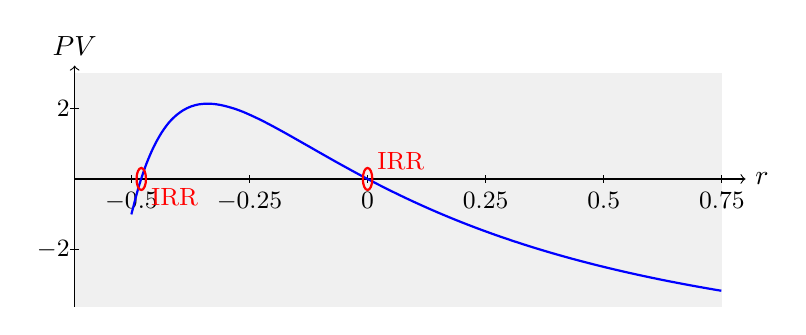
\begin{tikzpicture}[x=6cm, y=0.45cm]
        \fill[gray!12] (-0.62,-3.6) rectangle (0.75,3);
        \draw[->] (-0.62,0) -- (0.8,0) node[right] {$r$};
        \draw[->] (-0.62,-3.6) -- (-0.62,3.2) node[above] {$PV$};
        \foreach \x in {-0.5,-0.25,0,0.25,0.5,0.75} { \draw (\x,0.1) -- (\x,-0.1) node[below] {\small $\x$}; }
        \foreach \y in {-2,2} { \draw (-0.63,\y) -- (-0.61,\y) node[left] {\small $\y$}; }
        \draw[thick, blue, domain=-0.5:0.75, samples=80, smooth, variable=\r]
            plot ({\r}, {-5 - 2/(1+\r) + 12/(1+\r)^2 - 5/(1+\r)^3});
        \foreach \x in {-0.479,0} { \draw[red, thick] (\x,0) circle (0.06cm and 0.14cm); }
        \node[red, above right] at (0,0) {\small IRR};
        \node[red, below right] at (-0.479,0) {\small IRR};
    \end{tikzpicture}
    \end{center}
    $PV = 0$ at both $r = 0$ and $r \approx -0.48$, so this stream has \dbb{two IRRs}. The sign of the cash flows changes more than once, so the Main Theorem on IRR below does not apply.
\end{example}


\heading{Main Theorem on IRR}
Suppose the cash flow stream $x = (x_0, x_1, \dots, x_n)$ has $x_0 < 0$ and $x_k \geq 0$ for all $k > 0$, where at least one term is strictly positive. Then, there is a unique positive root to the equation
\[x_0+x_1c + x_2 c^2 + \dots + x_n c^n = 0\]
Proof: plot $f(c) = x_0 + x_1c + x_2c^2 + \dots + x_n c^n$

\begin{center}
\begin{tikzpicture}
    \draw[->] (-0.3,0) -- (4.5,0) node[right] {$c$};
    \draw[->] (0,-1.5) -- (0,1.8) node[above] {$f(c)$};
    \draw[thick, blue, domain=0:4, smooth, variable=\x] plot ({\x}, {-1 + 0.15*\x*\x});
    \draw[dashed] (2.58,0) -- (2.58,-1.5);
    \filldraw (2.58,0) circle (1.5pt);
    \node[below] at (2.58,-0.05) {$c^*$};
    \filldraw (0,-1) circle (1.5pt);
    \node[left] at (0,-1) {$x_0$};
\end{tikzpicture}
\end{center}
Since $f(0) = x_0 < 0$ and $f'(c) = x_1 + 2x_2c + \dots + nx_nc^{n-1} \geq 0$ for $c \geq 0$ (as each $x_k \geq 0$, with at least one strictly positive), $f$ is strictly increasing for $c > 0$ and unbounded above. So $f$ crosses zero exactly once, at some $c^* > 0$, giving the unique IRR $r = 1/c^* - 1 > -1$.

\heading{Net Present Value (NPV)}
Computes all present values of \textit{all} cash flows associated with an investment. Includes the investment term $x_0$ as well.

\begin{example}[When to Cut a Tree]
    You can plant trees to be sold for lumber later, with two options for when to cut (interest rate 10\%):
    \begin{enumerate}[label=(\arabic*)]
        \item After 1 year: $(-1,2)$
        \item After 2 years: $(-1,0, 3)$
    \end{enumerate}
    Using NPV (choose largest NPV):
    \[-1 + \frac{2}{1.1} = 0.82 \quad \text{vs} \quad -1 + \frac{0}{1.1} + \frac{3}{1.1^2} = 1.48\]
    NPV says choose option (2).
    \\Using IRR (choose greatest IRR):
    \[-1 + 2c = 0 \Rightarrow c = 0.5 \Rightarrow r = 1.0 \quad \text{vs} \quad -1+3c^2 = 0 \Rightarrow c = 0.577 \Rightarrow r = 0.7\]
    IRR says choose option (1).
\end{example}

\keypoint{IRR and NPV give conflicting recommendations.}
\keypoint{IRR is scale invariant, Present Value is not.\\PV distinguishes between single and repeated cash flows, IRR does not.}
In general, NPV is preferred.

\begin{example}
    Scaling and repetition (PV at 10\%):
    \begin{center}
    \begin{tabular}{lccc}
        \toprule
        Cash flows & $(-1,2)$ & $10\cdot(-1,2)$ & $(-1,2,-1,2,\dots)$\\
        \midrule
        PV & 0.818 & 8.18 & 4.71\\
        IRR & $r=1.0$ & $r=1.0$ & $r=1.0$\\
        \bottomrule
    \end{tabular}
    \end{center}
\end{example}

NPV is preferred because it distinguishes between more cash flows, but this means the cash flows and assumptions need to be modelled carefully before the NPV analysis is done. E.g. the tree-cutting NPV analysis assumes it is done only \textit{once}; if the process can be repeated many times, we arrive at a different answer. Methods of IRR analysis exist that make it agree with NPV (e.g. incremental IRR analysis).

\heading{Steps to Solving Cash Flow Problems}
\begin{enumerate}
    \item Write down the cash flow diagram for each alternative (include \textit{all} cash flows).
    \item Evaluate the NPV of each cash flow.
    \item Choose the alternative with the largest NPV.
\end{enumerate}

\heading{Cycle Problems}
Relate to activities that can be repeated. With NPV you arrive at a different answer depending on how many times an activity is repeated, so the activities must be evaluated over the \underline{same time horizon}. Two approaches:
\begin{enumerate}
    \item Repeat both activities until they terminate at the same time.
    \item Repeat both to infinity: for an activity with lifetime $T$ and one-cycle present value $PV_1$,
    \[PV_1\sum_{k=0}^{\infty}\frac{1}{(1+r)^{Tk}} = PV_1\cdot\frac{1}{1-\frac{1}{(1+r)^T}}\]
\end{enumerate}

\begin{example}[Refrigerator Purchase]
    Model A: price \$600, yearly cost \$180 (beginning of year), life 3 years.
    \\Model B: price \$800, yearly cost \$120 (beginning of year), life 5 years.
    \\Interest rate is 10\%. Over 15 years (costs drawn as arrows, tall arrows mark a new purchase):
    \begin{center}
    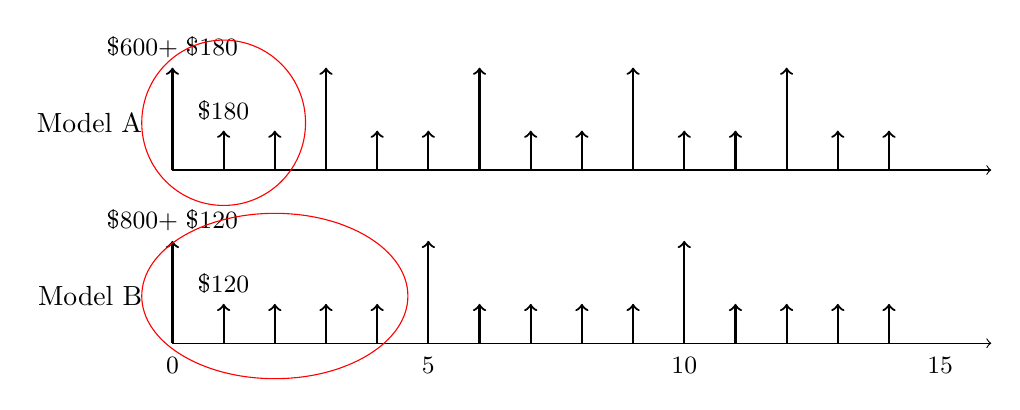
\begin{tikzpicture}[x=0.65cm]
        \foreach \row/\name/\life/\pr/\yc in {0/A/3/600/180, -2.2/B/5/800/120} {
            \begin{scope}[yshift=\row cm]
                \node[left] at (-0.4,0.6) {Model \name};
                \draw[->] (0,0) -- (16,0);
                \foreach \t in {0,...,14} {
                    \pgfmathtruncatemacro{\buy}{mod(\t,\life)==0}
                    \ifnum\buy=1 \draw[->, thick] (\t,0) -- (\t,1.3); \else \draw[->, thick] (\t,0) -- (\t,0.5); \fi
                }
                \node[above] at (0,1.3) {\small \$\pr + \$\yc};
                \node[above] at (1,0.5) {\small \$\yc};
                \draw[red] (\life/2-0.5,0.6) ellipse ({\life/2+0.1} and 1.05);
            \end{scope}
        }
        \foreach \t in {0,5,10,15} { \node[below] at (\t,-2.25) {\small \t}; }
    \end{tikzpicture}
    \end{center}
    One cycle of each (circled; price and first cost at time 0):
    \[PV_A = 780 + 180\sum_{k=1}^{2}\frac{1}{1.1^k} = \$1,092.40 \qquad PV_B = 920 + 120\sum_{k=1}^{4}\frac{1}{1.1^k} = \$1,300.38\]
    \b{Approach 1}: equal horizons, 15 years = 5 cycles of A = 3 cycles of B
    \begin{align*}
        A&: PV_A\left(1+\frac{1}{1.1^3}+\frac{1}{1.1^6}+\frac{1}{1.1^9}+\frac{1}{1.1^{12}}\right) = \$3,341.11\\
        B&: PV_B\left(1+\frac{1}{1.1^5}+\frac{1}{1.1^{10}}\right) = \$2,609.17
    \end{align*}
    \b{Approach 2}: repeat to infinity
    \begin{align*}
        A&: 1092.40\cdot\frac{1}{1-\frac{1}{1.1^3}} = \$4,392.70\\
        B&: 1300.38\cdot\frac{1}{1-\frac{1}{1.1^5}} = \$3,430.37
    \end{align*}
    These are costs, so the smaller is better: choose Model B in both approaches.
\end{example}

\heading{Summing Geometric Series}
\begin{align*}
    S = \sum_{k=0}^{\infty}x^k &= 1 + x + x^2 + \cdots\\
    &= 1 + x(1+x+x^2+\cdots) = 1 + xS
\end{align*}
\[S(1-x) = 1 \quad \Rightarrow \quad S = \frac{1}{1-x} \qquad (|x|<1)\]

% !TeX root = ../main.tex

\newlecture[Fixed Income Securities][Sep 21 \& 24, 2026]

\begin{definition}[Financial Instruments]
    A legal obligation or claim having monetary value (eg. mortgage, stocks and bonds...)
\end{definition}
\begin{definition}[Security]
    A tradable financial instrument satisfying legal and regulatory requirements.
\end{definition}
\begin{definition}[Fixed Income Securities]
    Securities that promise a fixed income to the holder over some span of time. (eg. bonds, mortgages, annuities)
\end{definition}

\heading{Annuity}
A contract that pays the holder money periodically according to the fixed schedule.
\\\b{Perpetual Annuity (Perpetuity)} - Pays a fixed sum periodically, forever.

\begin{center}
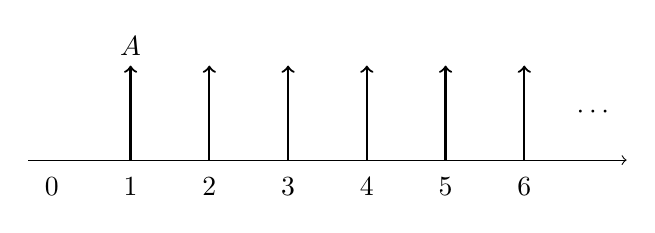
\begin{tikzpicture}
    \draw[->] (-0.3,0) -- (7.3,0);
    \foreach \x in {0,1,2,3,4,5,6} {
        \node[below] at (\x,-0.1) {\x};
    }
    \foreach \x in {1,2,3,4,5,6} {
        \draw[->, thick] (\x,0) -- (\x,1.2);
    }
    \node[above] at (1,1.2) {$A$};
    \node at (6.9,0.6) {$\cdots$};
\end{tikzpicture}
\end{center}

At a per period interest rate of $r$, the PV is
\[P = \sum_{k=1}^{\infty}\frac{A}{(1+r)^k} = \frac{A}{r}\]
Note: Infinite sum!!

\begin{example}
    A perpetual annuity of \$1,000 each year at 10\% interest/year has present value
    \[P = \frac{A}{r} = \frac{\$1,000}{0.1} = \$10,000\]
\end{example}


\heading{Finite-Life Streams}
A stream that pays $A$ for $n$ periods, starting at period 1. What is the PV?

\begin{center}
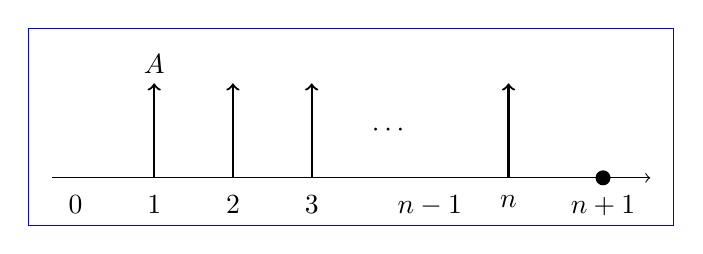
\begin{tikzpicture}
    \draw[blue] (-0.6,-0.6) rectangle (7.6,1.9);
    \draw[->] (-0.3,0) -- (7.3,0);
    \node[below] at (0,-0.1) {$0$};
    \node[below] at (1,-0.1) {$1$};
    \node[below] at (2,-0.1) {$2$};
    \node[below] at (3,-0.1) {$3$};
    \node[below] at (4.5,-0.1) {$n-1$};
    \node[below] at (5.5,-0.1) {$n$};
    \node[below] at (6.7,-0.1) {$n+1$};
    \draw[->, thick] (1,0) -- (1,1.2);
    \draw[->, thick] (2,0) -- (2,1.2);
    \draw[->, thick] (3,0) -- (3,1.2);
    \node at (4,0.6) {$\cdots$};
    \draw[->, thick] (5.5,0) -- (5.5,1.2);
    \filldraw (6.7,0) circle (2.5pt);
    \node[above] at (1,1.2) {$A$};
\end{tikzpicture}
\end{center}

\[\boxed{P = \sum_{k=1}^{n}\frac{A}{(1+r)^k} = \frac{A}{r}\left(1-\frac{1}{(1+r)^n}\right)}\]
where $r$ is the interest rate per period.

A finite life-stream can be thought as the \underline{difference between two perpetuities}.

Perpetuity starting at period 1:
\begin{center}
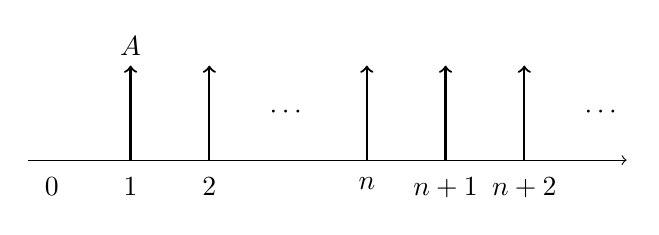
\begin{tikzpicture}
    \draw[->] (-0.3,0) -- (7.3,0);
    \node[below] at (0,-0.1) {$0$};
    \node[below] at (1,-0.1) {$1$};
    \node[below] at (2,-0.1) {$2$};
    \node[below] at (4,-0.1) {$n$};
    \node[below] at (5,-0.1) {$n+1$};
    \node[below] at (6,-0.1) {$n+2$};
    \draw[->, thick] (1,0) -- (1,1.2);
    \draw[->, thick] (2,0) -- (2,1.2);
    \draw[->, thick] (4,0) -- (4,1.2);
    \draw[->, thick] (5,0) -- (5,1.2);
    \draw[->, thick] (6,0) -- (6,1.2);
    \node at (3,0.6) {$\cdots$};
    \node at (7,0.6) {$\cdots$};
    \node[above] at (1,1.2) {$A$};
\end{tikzpicture}
\end{center}

Perpetuity starting at period $n+1$:
\begin{center}
\begin{tikzpicture}
    \draw[->] (-0.3,0) -- (7.3,0);
    \node[below] at (0,-0.1) {$0$};
    \node[below] at (1,-0.1) {$1$};
    \node[below] at (2,-0.1) {$2$};
    \node[below] at (4,-0.1) {$n$};
    \node[below] at (5,-0.1) {$n+1$};
    \node[below] at (6,-0.1) {$n+2$};
    \draw[->, thick] (5,0) -- (5,1.2);
    \draw[->, thick] (6,0) -- (6,1.2);
    \node at (3,0.6) {$\cdots$};
    \node at (7,0.6) {$\cdots$};
    \node[above] at (5,1.2) {$A$};
\end{tikzpicture}
\end{center}
\[PV = \frac{A}{r} - \frac{A}{r}\left(\frac{1}{(1+r)^n}\right)\]
\[PV_{fin} = \frac{A}{r}\left(1 - \frac{1}{(1+r)^n}\right)\]


\begin{example}[Loan Calculation]
    Suppose \$1,000 is borrowed at 12\% interest compounded monthly, repayed with equal monthly payments over 5 years. How much are the monthly payments?

    Given: $P = \$1,000 \quad r = \frac{12\%}{12} = 1\%/\text{mo} \quad n = 5\times12 = 60$
    \[P = \frac{A}{r}\left(1-\frac{1}{(1+r)^n}\right) \quad \Rightarrow \quad A = \frac{rP}{\left(1-\frac{1}{(1+r)^n}\right)} = \$22.24/\text{mo}\]
\end{example}

\header{Bonds}
An agreement to pay money according to the rules of the issue.
\\Generally, bonds have\begin{itemize}
    \item Face Value, Par Value, Principal - an amount to be paid at the maturity date.
    \item Coupon Payments - an amount paid periodically, expressed as a \% of the face value. Last coupon is paid at maturity.
\end{itemize}

\begin{example}
    Given:
    \[\text{Face Value } = \$1,000 \qquad \text{Coupon } = 9\%\]
    The yearly coupon amount is $\$1,000(0.09) = \$90$
\end{example}
In general, coupons are paid $m$ times per year, so each payment is $C/m$ where $C$ is the yearly coupon amount. In the U.S., coupons are usually paid every six months ($m=2$), e.g. US treasury bonds with this example pay \$45 every 6 months (\$90/2).

\header{Payoff Structure of a Bond}
\begin{center}
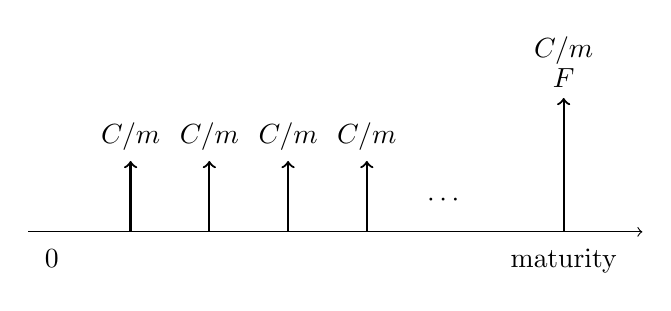
\begin{tikzpicture}
    \draw[->] (-0.3,0) -- (7.5,0);
    \node[below] at (0,-0.1) {$0$};
    \node[below] at (6.5,-0.1) {maturity};
    \draw[->, thick] (1,0) -- (1,0.9) node[above] {$C/m$};
    \draw[->, thick] (2,0) -- (2,0.9) node[above] {$C/m$};
    \draw[->, thick] (3,0) -- (3,0.9) node[above] {$C/m$};
    \draw[->, thick] (4,0) -- (4,0.9) node[above] {$C/m$};
    \node at (5,0.4) {$\cdots$};
    \draw[->, thick] (6.5,0) -- (6.5,1.7);
    \node at (6.5,2.3) {$C/m$};
    \node at (6.5,1.95) {$F$};
\end{tikzpicture}
\end{center}

where $C$ is the annual coupon amount, and $F$ is the face value.

When there are no coupons, the only payoff is the face value at maturity.

\begin{center}
\begin{tikzpicture}
    \draw[->] (-0.3,0) -- (7.5,0);
    \node[below] at (0,-0.1) {$0$};
    \node[below] at (6.5,-0.1) {maturity};
    \node at (3.5,0.4) {$\cdots$};
    \draw[->, thick] (6.5,0) -- (6.5,1.2) node[above] {$F$};
\end{tikzpicture}
\end{center}

This is known as a \b{zero-coupon bond}, or a zero.

\header{Accrued Interest}
Ignored by bond price quotes, but must be added to the price.

\begin{center}
\begin{tikzpicture}
    \draw[->] (-0.3,0) -- (8.5,0);
    \draw[->, thick] (0,0) -- (0,1.3) node[above] {$C/m$};
    \draw[->, thick] (8,0) -- (8,1.3) node[above] {$C/m$};
    \draw[decorate, decoration={brace, amplitude=6pt}] (0.3,0.85) -- (7.7,0.85) node[midway, above=8pt] {$t_c$};
    \draw[decorate, decoration={brace, mirror, amplitude=6pt}] (0,-0.3) -- (5,-0.3) node[midway, below=8pt] {$t$};
    \draw[->] (6.2,-1.6) -- (5.1,-0.2);
    \node[below] at (6.6,-1.7) {you purchase};
\end{tikzpicture}
\end{center}

You must pay the previous owner their ``portion'' of the next coupon payment.

\[\boxed{AI = \frac{\text{days since last coupon}}{\text{days in current coupon period}} \times (C/m) = \frac{t}{t_c}(C/m)}\]

\begin{example}
    A treasury bond is purchased on May 8 and matures on August 15 in some future year. The coupon rate is 9\% and coupons are paid every Feb 15 and Aug 15. How much accrued interest is owed?
    \\On May 8th, 83 days have passed since the last coupon and 99 days remain until the next. With $C/m = 9\%/2 = 4.5\%$:
    \[AI = \frac{83}{83+99}\times 4.5\% = 2.05\%\]
\end{example}

\begin{definition}
    \rb{Clean price}: the market bond price (quoted, doesn't include accrued interest).
    \\\rb{Dirty (cash) price}: the clean price plus accrued interest, i.e. what you actually pay.
\end{definition}

\b{Government Securities}:
\begin{itemize}
    \item Bill: up to 1 year
    \item Note: 1 to 10 years
    \item Bond: 10 to 30 years
\end{itemize}

\header{Bond Price and Yield}
The whole cash flow stream of purchasing a bond can be mapped out, where $P$ is the entire amount paid for the bond: the market price plus accrued interest (the dirty price).

\begin{center}
\begin{tikzpicture}
    \draw[->] (-0.3,0) -- (7.5,0);
    \node[above left] at (0,0) {$0$};
    \node[below] at (6.5,0) {$n$};
    \draw[->, thick] (0,0) -- (0,-1.2) node[below] {$P$};
    \draw[->, thick] (1,0) -- (1,0.9) node[above] {$C/m$};
    \draw[->, thick] (2,0) -- (2,0.9) node[above] {$C/m$};
    \draw[->, thick] (3,0) -- (3,0.9) node[above] {$C/m$};
    \draw[->, thick] (4,0) -- (4,0.9) node[above] {$C/m$};
    \node at (5.2,0.4) {$\cdots$};
    \draw[->, thick] (6.5,0) -- (6.5,1.7);
    \node at (6.5,2.3) {$C/m$};
    \node at (6.5,1.95) {$F$};
\end{tikzpicture}
\end{center}

The IRR of this cash flow stream is the \rb{yield} (or \rb{yield to maturity}) of the bond, denoted $\lambda$. It captures the rate of return from buying the bond and holding it to maturity.

\[\boxed{\begin{gathered}
    P = \underbrace{\frac{F}{\left(1+\frac{\lambda}{m}\right)^n}}_{\text{PV of face}} + \underbrace{\frac{C/m}{\lambda/m}\left[1-\frac{1}{\left(1+\frac{\lambda}{m}\right)^n}\right]}_{\text{annuity formula}}\\[4pt]
    \begin{array}{@{}l@{}}
        P: \text{price including accrued interest}\\
        F: \text{face value}\\
        m: \text{coupon payments per year (compounding $m$ times per year)}\\
        C/m: \text{amount of each coupon payment}\\
        \lambda/m: \text{yield per coupon period}\\
        n: \text{coupon payments remaining}
    \end{array}
\end{gathered}}\]
Note this equation \underline{only} holds when $\lambda$ is the yield, with \underline{exactly} $n$ coupon payments remaining.

\begin{example}
    Price of a bond with par value \$1,000 paid in ten years, coupon rate 10\%, yield 12\%, coupons paid semi-annually. Then $n = 20$, $C/m = 50$, $\lambda/m = 6\%$:
    \[P = 50\cdot\frac{1-\frac{1}{(1.06)^{20}}}{0.06} + \frac{1000}{(1.06)^{20}} = 50(11.47) + 311.80 \approx \$885.30\]
\end{example}

\begin{definition}
    Comparing a bond's price $P$ to its face value $F$ (equivalently, its coupon rate $C/F$ to its yield $\lambda$):
    \begin{itemize}
        \item \rb{Par bond}: $P = F$, when the coupon rate \dbb{equals} the yield.
        \item \rb{Premium bond}: $P > F$, when the coupon rate is \dbb{above} the yield.
        \item \rb{Discount bond}: $P < F$, when the coupon rate is \dbb{below} the yield.
    \end{itemize}
\end{definition}
E.g.\ the bond above has a 10\% coupon but a 12\% yield, so it sells at a discount ($\$885.30 < \$1,000$).

\header{The Price-Yield Curve}
For a fixed maturity, \underline{price and yield are inversly related}:
\begin{itemize}
    \item Rates Rise $\rightarrow$ Existing bond prices Fall
    \item Rates Fall $\rightarrow$ Existing bond prices Rise
\end{itemize}
The longer the time to maturity, the more sensitive the price of the bond is to the yield.

\begin{center}
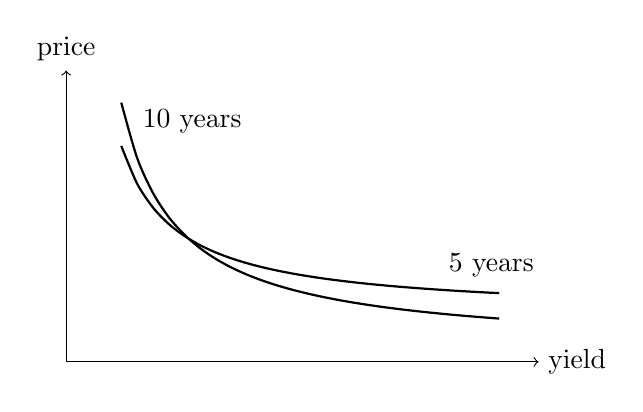
\begin{tikzpicture}
    \draw[->] (0,0) -- (6,0) node[right] {yield};
    \draw[->] (0,0) -- (0,3.7) node[above] {price};
    \draw[thick, domain=0.7:5.5, smooth, variable=\x] plot ({\x}, {0.6 + 1.5/\x});
    \draw[thick, domain=0.7:5.5, smooth, variable=\x] plot ({\x}, {0.15 + 2.2/\x});
    \node[right] at (0.85,3.05) {10 years};
    \node[above] at (5.4,0.95) {5 years};
\end{tikzpicture}
\end{center}

\begin{example}
    A 30-year zero-coupon bond with face value \$1,000, priced at different yields:
    \begin{center}
    \begin{tabular}{lcccccc}
        \toprule
        Yield & 1\% & 2\% & 5\% & 10\% & 15\% & 20\%\\
        \midrule
        Price & \$741.37 & \$550.45 & \$227.28 & \$53.54 & \$13.05 & \$3.28\\
        \bottomrule
    \end{tabular}
    \end{center}
    Price falls steeply as yield rises: $P = 1000/(1+\lambda)^{30}$.
\end{example}

The \b{current yield} is the coupon divided by the current price. In this course, \dbb{yield} always means \dbb{yield to maturity}.

\begin{example}[Bond Quote]
    Treasury quotes from yahoo.com (YTM = yield to maturity, CY = current yield):
    \begin{center}
    \begin{tabular}{lcccc}
        \toprule
        Issue & Price & Coupon & YTM & CY\\
        \midrule
        T-Note, matures 31-Oct-2005 & 99.91 & 1.625 & 2.923 & 1.626\\
        T-Note, matures 15-Jan-2011 & 109.71 & 3.500 & 1.574 & 3.190\\
        T-Bond, matures 15-Feb-2021 & 135.49 & 7.875 & 4.622 & 5.812\\
        \bottomrule
    \end{tabular}
    \end{center}
    Check: $CY = 7.875/135.49 = 5.812\%$. YTM and CY can differ a lot, since CY ignores the face value repaid at maturity.
\end{example}

\noindent\begin{minipage}{\textwidth}
\header{Bond Ratings}
Standard \& Poor's and Moody's are two independent bond rating agencies.
\begin{center}
\begin{tabular}{@{}llll@{}}
    \toprule
    & S\&P & Moody's & Meaning\\
    \midrule
    Investment & AAA & Aaa & Best quality, smallest credit risk (US gov. bonds)\\
    Grade & AA & Aa & High grade\\
    & A & A & High to medium grade\\
    & BBB & Baa & Medium grade\\
    \midrule
    Speculative & BB & Ba & Judged to be speculative\\
    Grade & B & B & Increasingly speculative\\
    (Junk Bonds) & CCC & Caa & Danger of default\\
    & CC & Ca & Very speculative, high chance of default\\
    & C & C & Small chance of not defaulting\\
    & D & D & In default\\
    \bottomrule
\end{tabular}
\end{center}
\end{minipage}
\par

% !TeX root = ../main.tex

\newlecture[The Term Structure of Interest Rates][Sep 28, 2026]

\header{The Yield Curve}
In general, yields on bonds of different maturities are different, i.e. \ul{interest rates are a function of time}.
\\Plotting yield vs.\ time to maturity for bonds gives the \rb{yield curve}.

\begin{center}
\begin{tikzpicture}
    \draw[->] (0,0) -- (6,0) node[right] {time to maturity};
    \draw[->] (0,0) -- (0,3) node[above] {yield};
    \draw[thick, domain=0.2:5.3, smooth, variable=\x] plot ({\x}, {2.4 - 1.4*exp(-0.7*\x)});
\end{tikzpicture}
\end{center}

Real U.S.\ Treasury yield curves (yahoo.com): on Sep 10, 2004 the curve rose steeply from about 1.5\% (3 months) to 5\% (30 years); on Oct 4, 2005 it was much flatter, from about 3.5\% to 4.6\%. The \ul{shape of the curve changes over time}.

The yield curve is not exactly what we want, since bonds may have coupons (intermediate cash flows). We would really like to know the interest rate on a \dbb{single cash flow at time $t$}, with no intermediate cash flows.

\begin{center}
\begin{tikzpicture}
    \draw[->] (-0.3,0) -- (5,0);
    \node[below] at (0,-0.1) {$0$};
    \node[below] at (4,-0.1) {$t$};
    \draw[->, thick] (4,0) -- (4,1.2);
\end{tikzpicture}
\end{center}

\header{Spot Rates}
\begin{definition}[Spot Rate]
    Interest rates for a specific time $t$. Always \dbb{annual nominal interest rates}, can be compounded yearly, $m$ periods per year, or continuously.
\end{definition}

\begin{framed}
\begin{center}
\begin{tikzpicture}
    \draw[->] (0,0) -- (6,0) node[right] {time};
    \draw[->] (0,0) -- (0,3) node[above] {spot rate};
    \draw[thick, domain=0.2:5.3, smooth, variable=\x] plot ({\x}, {2.4 - 1.4*exp(-0.7*\x)});
\end{tikzpicture}
\end{center}

Plotting spot rates vs.\ time gives the \rb{spot rate curve}, also known as the \rb{term structure of interest rates}.
\\We can price bonds reliably with predictions through the term structure of interest (quant!!).
\end{framed}


\heading{Present Value and Spot Rates}
When computing present value, the \ul{spot rate corresponding to the time of each cash flow} must be used for discounting:
\[\boxed{PV = x_0 + \frac{x_1}{1+s_1} + \frac{x_2}{(1+s_2)^2} + \cdots + \frac{x_n}{(1+s_n)^n}}\]

\begin{example}
    \begin{center}
    \begin{tikzpicture}
        \draw[->] (-0.3,0) -- (5,0);
        \foreach \x in {0,1,2,3,4} {
            \draw (\x,0.05) -- (\x,-0.05);
        }
        \draw[->, thick] (0,0) -- (0,-0.6) node[below] {$-1$};
        \draw[->, thick] (1,0) -- (1,1.2) node[above] {$2$};
        \draw[->, thick] (2,0) -- (2,0.6) node[above] {$1$};
        \draw[->, thick] (3,0) -- (3,-1.2) node[below] {$-2$};
        \draw[->, thick] (4,0) -- (4,0.6) node[above] {$1$};
    \end{tikzpicture}
    \end{center}
    \begin{center}
    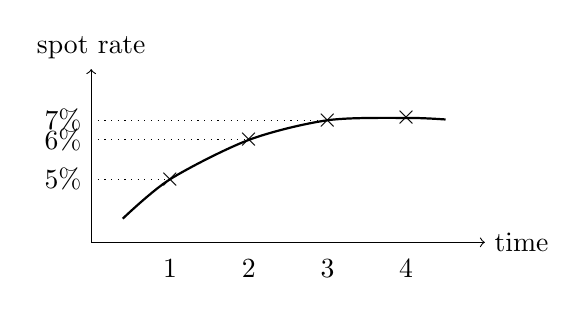
\begin{tikzpicture}
        \draw[->] (0,0) -- (5,0) node[right] {time};
        \draw[->] (0,0) -- (0,2.2) node[above] {spot rate};
        \foreach \x in {1,2,3,4} {
            \node[below] at (\x,-0.1) {\x};
        }
        \draw[thick, smooth] plot coordinates {(0.4,0.3) (1,0.8) (2,1.3) (3,1.55) (4,1.58) (4.5,1.56)};
        \foreach \x/\y/\r in {1/0.8/5, 2/1.3/6, 3/1.55/7} {
            \draw[dotted] (0,\y) -- (\x,\y);
            \node[left] at (0,\y) {\r\%};
        }
        \foreach \x/\y in {1/0.8, 2/1.3, 3/1.55, 4/1.58} {
            \node at (\x,\y) {$\times$};
        }
    \end{tikzpicture}
    \end{center}
    \begin{center}
    \begin{tabular}{lccccc}
        \toprule
        Time & 0 & 1 & 2 & 3 & 4\\
        \midrule
        Cash flow & $-1$ & 2 & 1 & $-2$ & 1\\
        Spot rate & & 5\% & 6\% & 7\% & 7\%\\
        \bottomrule
    \end{tabular}
    \end{center}
    \[PV = -1 + \frac{2}{1.05} + \frac{1}{1.06^2} + \frac{-2}{1.07^3} + \frac{1}{1.07^4} = 0.925\]
\end{example}

\heading{Determining Spot Rates}
If you know the price of a \dbb{zero-coupon bond}, \ul{its yield is the spot rate}. Given price $P$ and face value $F$ of a zero maturing at $t$:
\[\boxed{P = Fe^{-s_t t}} \quad \text{(continuous compounding)} \qquad \boxed{P = \frac{F}{(1+s_t)^t}} \quad \text{(discrete compounding)}\]
\b{Problem}: What if there are no zeros?
\\\b{Solution}: Construct a zero-coupon bond from coupon bonds.

\header{Constructing Zeros}
Take two coupon bonds with the same maturity (and coupon dates) and form a portfolio of $x$ of bond 1 and $y$ of bond 2 (negative means short).

\begin{center}
\begin{tikzpicture}
    \node[left] at (-0.5,0.5) {Bond $i$};
    \draw[->] (-0.3,0) -- (7.5,0);
    \node[above left] at (0,0) {$0$};
    \node[below] at (6.5,0) {maturity};
    \draw[->, thick] (0,0) -- (0,-1) node[below] {$P_i$};
    \draw[->, thick] (1,0) -- (1,0.9) node[above] {$C_i$};
    \draw[->, thick] (2,0) -- (2,0.9) node[above] {$C_i$};
    \draw[->, thick] (3,0) -- (3,0.9) node[above] {$C_i$};
    \draw[->, thick] (4,0) -- (4,0.9) node[above] {$C_i$};
    \node at (5.2,0.4) {$\cdots$};
    \draw[->, thick] (6.5,0) -- (6.5,1.7);
    \node at (6.5,2.3) {$C_i$};
    \node at (6.5,1.95) {$F_i$};
\end{tikzpicture}
\end{center}

Three equations for the portfolio:
\[\boxed{\begin{aligned}
    \text{Coupon:} &\quad xC_1 + yC_2 = C_0 \\
    \text{Face:} &\quad xF_1 + yF_2 = F_0 \\
    \text{Price:} &\quad xP_1 + yP_2 = P_0
\end{aligned}}\]
To construct a zero, set $C_0 = 0$ and $F_0 = \$100$, assuming $F_0 = F_1 = F_2$. Then solve for $x$ and $y$. 
\\The price of the zero is then $P_0 = xP_1 + yP_2$, and the spot rate could be computed.

\begin{example}
    Portfolio of 3 of bond 1 (face \$100, 10\% coupon) and $-2.5$ of bond 2 (face \$100, 12\% coupon), both maturing at $t=5$:
    \begin{center}
    \begin{tabular}{lcccc}
        \toprule
        Time & 0.5 & 1 & $\cdots$ & 5\\
        \midrule
        Bond 1 & 10 & 10 & $\cdots$ & 110\\
        Bond 2 & 12 & 12 & $\cdots$ & 112\\
        Portfolio & 0 & 0 & $\cdots$ & 50\\
        \bottomrule
    \end{tabular}
    \end{center}
    Coupons cancel: $3(10) - 2.5(12) = 0$, leaving only $3(110) - 2.5(112) = 50$ at maturity, a zero.
\end{example}

\begin{example}
    Bond 1: 10 year, 10\% coupon, $P_1 = \$98.72$. Bond 2: 10 year, 8\% coupon, $P_2 = \$85.89$.
    \\(Note: Choose two bonds with the \dbb{same maturity}, so the spot rate for that maturity can be computed)
    \\Create a zero:
    \[\begin{cases}
        \text{Coupon:} & 10x + 8y = 0\\
        \text{Face:} & 100x + 100y = 100
    \end{cases} \quad \Rightarrow \quad x = -4,\ y = 5\]
    Price of zero: $xP_1 + yP_2 = -4(98.72) + 5(85.89) = \$34.57$
    \\Spot Rate (discrete compounding):
    \[34.57 = \frac{100}{(1+s_{10})^{10}} \quad \Rightarrow \quad s_{10} = 0.112 = 11.2\%\]
    Note: if possible, you can compare this computed value with the actual yield, then see which one is "better"
\end{example}

\header{Forward Rates}
\begin{definition}[\rb{Forward Rates}]
    The interest rate for money to be borrowed between two dates \ul{in the future}, but under terms \ul{agreed upon today}. 
    \[f_{t_1,t_2}: \text{the forward rate between $t_1$ and $t_2$.}\]
    Note: $t_1$ can be 0, but not negative, when $t_1 = 0$, $f_{0, t_2} = $ to the spot rate of $t_2$.
\end{definition}
How can forward rates be computed from the spot rate curve?

Starting with \$1 at time 1 and moving it to time 2, we should have $1+f_{1,2}$ by the definition of the forward rate. Spot rates tell us how to move money to and from time 0, so we can instead go \ul{through time 0}:

\begin{center}
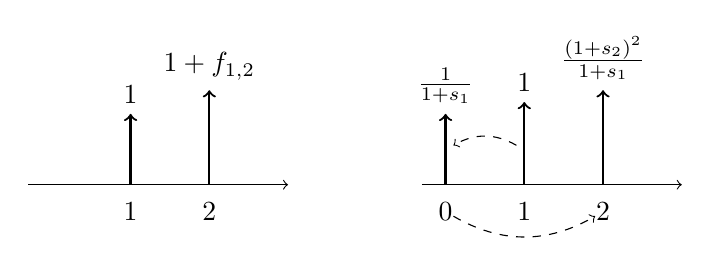
\begin{tikzpicture}
    % direct
    \draw[->] (-0.3,0) -- (3,0);
    \node[below] at (1,-0.1) {$1$};
    \node[below] at (2,-0.1) {$2$};
    \draw[->, thick] (1,0) -- (1,0.9) node[above] {$1$};
    \draw[->, thick] (2,0) -- (2,1.2) node[above] {$1+f_{1,2}$};
    % via time 0
    \begin{scope}[xshift=5cm]
        \draw[->] (-0.3,0) -- (3,0);
        \node[below] at (0,-0.1) {$0$};
        \node[below] at (1,-0.1) {$1$};
        \node[below] at (2,-0.1) {$2$};
        \draw[->, thick] (0,0) -- (0,0.9) node[above] {$\frac{1}{1+s_1}$};
        \draw[->, thick] (1,0) -- (1, 1.05) node[above] {$1$};
        \draw[->, thick] (2,0) -- (2,1.2) node[above] {$\frac{(1+s_2)^2}{1+s_1}$};
        \draw[->, dashed] (0.9,0.5) to[bend right] (0.1,0.5);
        \draw[->, dashed] (0.1,-0.4) to[bend right] (1.9,-0.4);
    \end{scope}
\end{tikzpicture}
\end{center}

\[1+f_{1,2} = \frac{(1+s_2)^2}{1+s_1} \quad \Rightarrow \quad \boxed{f_{1,2} = \frac{(1+s_2)^2}{1+s_1} - 1}\]

\begin{example}
    Spot rates for 1 and 2 years are 7\% and 8\%. The implied forward rate is
    \[f_{1,2} = \frac{(1.08)^2}{1.07} - 1 = 0.0901\]
    Note that the forward rate has to be \dbb{larger} than 8\% to balance out the \((1+0.0.8)^2\)
\end{example}

\heading{Formula for Forward Rates}
Invest \$1 at time 0 until time $j$ in two ways: (1) at the spot rate $s_i$ until $i$, then at the forward rate $f_{i,j}$ until $j$; (2) directly at the spot rate $s_j$. Both must give the same result:

\begin{center}
\begin{tikzpicture}
    % (1) via time i
    \node at (1.6,1.6) {(1) through $i$};
    \foreach \row/\t/\h/\lab in {0/0/0.8/{$1$}, -1.9/1.5/0.8/{$(1+s_i)^i$}, -3.8/3/0.8/{$(1+s_i)^i(1+f_{i,j})^{j-i}$}} {
        \begin{scope}[yshift=\row cm]
            \draw[->] (-0.3,0) -- (4,0);
            \node[below] at (0,-0.05) {$0$};
            \node[below] at (1.5,-0.05) {$i$};
            \node[below] at (3,-0.05) {$j$};
            \draw[->, thick] (\t,0) -- (\t,\h) node[above] {\lab};
        \end{scope}
    }
    \draw[->, dashed] (0.3,-0.5) -- (1.2,-1.1);
    \draw[->, dashed] (1.8,-2.4) -- (2.7,-3.0);
    % divider
    \draw[blue] (5.2,1.8) -- (5.2,-4.3);
    % (2) direct
    \begin{scope}[xshift=6.4cm]
        \node at (1.6,1.6) {(2) directly};
        \foreach \row/\t/\lab in {0/0/{$1$}, -3.8/3/{$(1+s_j)^j$}} {
            \begin{scope}[yshift=\row cm]
                \draw[->] (-0.3,0) -- (4,0);
                \node[below] at (0,-0.05) {$0$};
                \node[below] at (1.5,-0.05) {$i$};
                \node[below] at (3,-0.05) {$j$};
                \draw[->, thick] (\t,0) -- (\t,0.8) node[above] {\lab};
            \end{scope}
        }
        \draw[->, dashed] (0.3,-0.5) -- (2.7,-3.0);
    \end{scope}
\end{tikzpicture}
\end{center}
\[\boxed{(1+s_i)^i(1+f_{i,j})^{j-i} = (1+s_j)^j} \qquad f_{i,j} = \left[\frac{(1+s_j)^j}{(1+s_i)^i}\right]^{1/(j-i)} - 1\]
Note: this calculation must be \ul{consistent with the type of compounding}.

\begin{example}
    Spot rates for 2 and 6 years are 3\% and 5\%. The implied forward rate is
    \[(1+s_2)^2(1+f_{2,6})^4 = (1+s_6)^6 \quad \Rightarrow \quad f_{2,6} = \left(\frac{(1.05)^6}{(1.03)^2}\right)^{1/4} - 1 = 6.01\%\]
\end{example}

\begin{definition}
    Rates that span only 1 period are \rb{short rates}. E.g.\ for yearly compounding: $s_1, f_{1,2}, f_{2,3}, \dots$
\end{definition}
Short rates can be determined from the spot rate curve and vice versa.

\header{Term Structure Explanations}
Why isn't the term structure (spot rate curve) flat? Three explanations:
\begin{enumerate}[label=(\arabic*)]
    \item \b{Expectations Theory}: spot rates are determined by the expectations of what interest rates will be. E.g.\ if the spot rate curve slopes upward, it is because people expect interest rates to increase in the future.
    \item \b{Liquidity Preference}: investors prefer short term securities over long term ones, since long term securities ``tie up'' money for long. There are also secure investments that are both easy to get in and out of.
    \item \b{Market Segmentation}: the fixed income market is segmented by maturity dates. The rate for each maturity is determined by the group of investors interested in that maturity, i.e.\ simple supply and demand among those investors.
\end{enumerate}

\header{Expectation Dynamics}
Forward rates are rates in the future that are agreed upon \rb{now}. But we don't know what the \dbb{actual future rates} will be when that time arrives, since spot rate curves could change.
When forward rates are used as a prediction (could be wrong) of the actual future rates, this forecast is called \rb{expectation dynamics}.
\\Prohibits arbitrage, using forward rates that are anchored on the spot rates today.

\heading{The Invariance Theorem}
If interest rates evolve according to expectation dynamics, then a sum of money invested in the interest rate market for $n$ years, will grow by a factor of $(1+s_n)^n$ \ul{regardless of the investment and reinvestment strategy} (no matter what combination of spot and forward rates).

\begin{center}
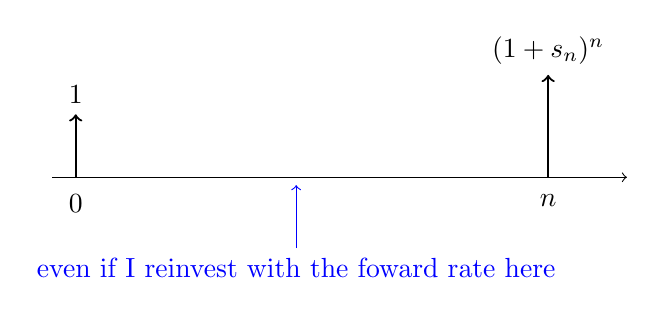
\begin{tikzpicture}
    \draw[->] (-0.3,0) -- (7,0);
    \node[below] at (0,-0.1) {$0$};
    \node[below] at (6,-0.1) {$n$};
    \draw[->, thick] (0,0) -- (0,0.8) node[above] {$1$};
    \draw[->, thick] (6,0) -- (6,1.3) node[above] {$(1+s_n)^n$};
    \draw[->, blue] (2.8,-0.9) -- (2.8,-0.1);
    \node[blue, below] at (2.8,-0.9) {even if I reinvest with the foward rate here};
\end{tikzpicture}
\end{center}

\b{Why?} Implied forward rates were \ul{computed to satisfy exactly this relationship}.
\\So even if you don't lock in a future interest rate now, you can still use forward rates for discounting, \ul{as long as you assume expectation dynamics}.


If expectation dynamics are assumed, the invariance thoerem is true (will always equal the same return value regardless of investment strategies.)
\newlecture[???he dindt post it yet so idk][Oct 1, 2026]

\header{Cash Matching Problem}
A series of future obligations must be met.
\\You have various bonds you can invest in, where the portfolio could be used to meet the obligation.
\\Choose portfolio of minimum cost that has enough money to meet the obligation (optimization!!)

Assumptions:
\begin{enumerate}[label = \arabic*)]
    \item No reinvestment of excess cash is allowed.
    \item Excess cash can be held at zero interest fron one period to the next.
    \item Excess cash can be reinvested at the appropriate forward rate.
\end{enumerate}

Constrained optimization?????

Note \# of bonds should always be non-negative!
$z_i$ is the possible excess cash generated, when positive, could be carried forward for reinvestment

Model 2 will never be worse than model one, worst case the same (z=0) than model 1, thus it is superior.

Model 3: investment with forward rate.
% !TeX root = ../main.tex

\newlecture[Bond Price Sensitivity][Oct 5, 2026]

Bond price sensitivity is measured two ways:
\begin{itemize}
    \item \b{Yield sensitivity}: Macaulay duration, modified duration, and the connection between them.
    \item \b{Spot rate curve sensitivity}: Fisher-Weil duration and quasi-modified duration.
\end{itemize}

\b{Question}: I would like to invest in a bond, but I am worried that bond yields may change in the future. Should I invest in a short or long maturity bond to reduce the effect of yield changes on the value of my bond? Should I choose a bond with large or small coupons?
\\\b{Answer}: We need a way to compute the \dbb{sensitivity of bond prices to yield/interest}.

\header{Sensitivity Related to Time to Maturity}
\begin{center}
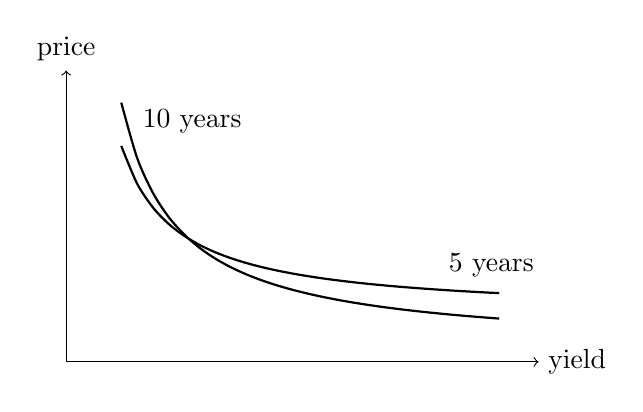
\begin{tikzpicture}
    \draw[->] (0,0) -- (6,0) node[right] {yield};
    \draw[->] (0,0) -- (0,3.7) node[above] {price};
    \draw[thick, domain=0.7:5.5, smooth, variable=\x] plot ({\x}, {0.6 + 1.5/\x});
    \draw[thick, domain=0.7:5.5, smooth, variable=\x] plot ({\x}, {0.15 + 2.2/\x});
    \node[right] at (0.85,3.05) {10 years};
    \node[above] at (5.4,0.95) {5 years};
\end{tikzpicture}
\end{center}
\keypoint{The longer the time to maturity, the more sensitive the price of the bond is to the yield.}

\header{Duration}
Maturity time is related to the sensitivity of the bond price to its yield.
\\In the case of zero-coupon bonds, the \rb{duration} (numerical measure for sensitivity) is the maturity (time measure), as the center of gravity is completely on the singular cash flow at maturity.
\\When there are coupons, the relationship is no longer direct.

\heading{Macaulay Duration}
Take the \dbb{weighted average} of the times to the cash flows, where each cash flow is weighted by its \dbb{present value} (computed with the yield) divided by the total present value.

\begin{center}
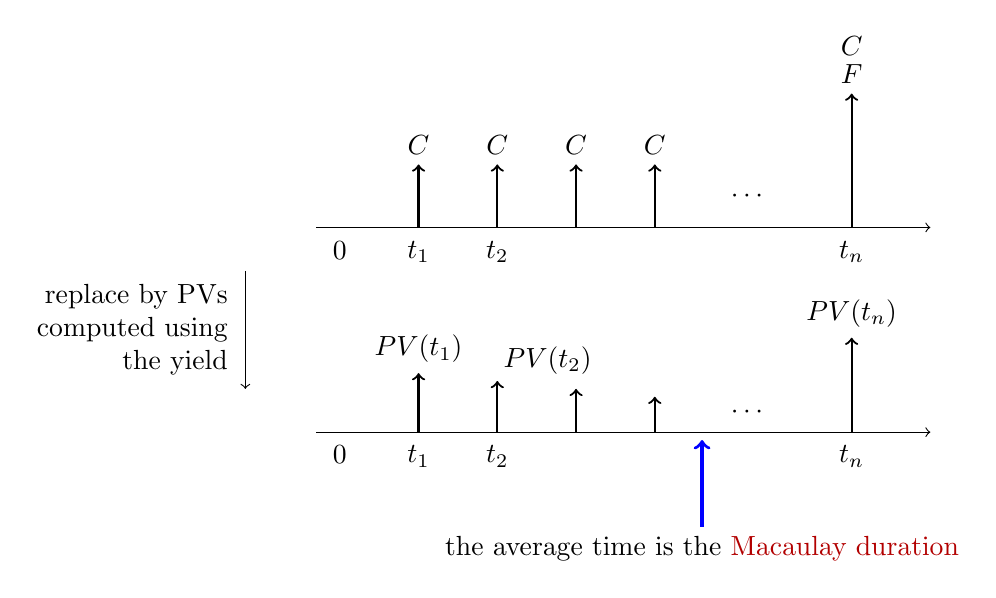
\begin{tikzpicture}
    % original cash flows
    \draw[->] (-0.3,0) -- (7.5,0);
    \node[below] at (0,-0.05) {$0$};
    \node[below] at (1,-0.05) {$t_1$};
    \node[below] at (2,-0.05) {$t_2$};
    \node[below] at (6.5,-0.05) {$t_n$};
    \foreach \x in {1,2,3,4} {
        \draw[->, thick] (\x,0) -- (\x,0.8) node[above] {$C$};
    }
    \node at (5.2,0.4) {$\cdots$};
    \draw[->, thick] (6.5,0) -- (6.5,1.7);
    \node at (6.5,2.3) {$C$};
    \node at (6.5,1.95) {$F$};
    % present values
    \begin{scope}[yshift=-2.6cm]
        \draw[->] (-0.3,0) -- (7.5,0);
        \node[below] at (0,-0.05) {$0$};
        \node[below] at (1,-0.05) {$t_1$};
        \node[below] at (2,-0.05) {$t_2$};
        \node[below] at (6.5,-0.05) {$t_n$};
        \draw[->, thick] (1,0) -- (1,0.75) node[above] {$PV(t_1)$};
        \draw[->, thick] (2,0) -- (2,0.65) node[above right=-2pt] {$PV(t_2)$};
        \draw[->, thick] (3,0) -- (3,0.55);
        \draw[->, thick] (4,0) -- (4,0.45);
        \node at (5.2,0.25) {$\cdots$};
        \draw[->, thick] (6.5,0) -- (6.5,1.2) node[above] {$PV(t_n)$};
        \draw[->, very thick, blue] (4.6,-1.2) -- (4.6,-0.1);
        \node[below, align=center] at (4.6,-1.2) {the average time is the \textcolor{red!70!black}{Macaulay duration}};
    \end{scope}
    \draw[->] (-1.2,-0.55) -- (-1.2,-2.05);
    \node[left, align=right] at (-1.3,-1.3) {replace by PVs\\computed using\\the yield};
\end{tikzpicture}
\end{center}

\begin{definition}[\rb{Macaulay Duration}]
    \[\boxed{\begin{aligned}
        D &= \frac{PV(t_1)t_1 + PV(t_2)t_2 + \cdots + PV(t_n)t_n}{PV_{total}}\\
        &= w_{t_1}t_1 + w_{t_2}t_2 + \cdots + w_{t_n}t_n\\
        &\text{where } w_{t_i} = \frac{PV(t_i)}{PV_{total}}
    \end{aligned}}\]
    Where $PV(t_i)$ is the present value of the cash flow at time $t_i$, computed \ul{using the yield as the interest rate}, and $PV_{total} = \sum_{i} PV(t_i)$ is the present value of the entire cash flow.
    \\Macaulay duration is a \dbb{weighted average of times}, so it is quoted in \dbb{years}. 
\end{definition}
\b{Economic meaning}: imagine buying a bond today. Macaulay duration answers ``if I view all future payments as one equivalent payment, at what average future date would I receive it?'' It is an \dbb{average waiting time to receiving cash}.

\heading{Macaulay Duration and Maturity}
\begin{itemize}
    \item Zero-coupon bond: Macaulay duration $=$ maturity date.
    \item Coupon bond: Macaulay duration $<$ maturity date.
\end{itemize}
\keypoint{\db{You should think}: a bond with \rb{Macaulay duration $D$} has the same yield sensitivity as a \rb{zero-coupon bond with maturity $D$}.}
Back to the opening question: to reduce the effect of yield changes, choose a bond with a \dbb{shorter maturity} and \dbb{larger coupons}, since both pull the duration down (larger coupons put more PV weight on earlier times).

\heading{Macaulay Duration Formula}
For a coupon bond:
\[\boxed{\begin{gathered}
    D = \frac{1+\frac{\lambda}{m}}{\lambda} - \frac{1 + \frac{\lambda}{m} + n\left(\frac{c}{m} - \frac{\lambda}{m}\right)}{c\left[\left(1+\frac{\lambda}{m}\right)^n - 1\right] + \lambda}\\[4pt]
    \begin{array}{@{}l@{}}
        c: \text{coupon rate per year}\\
        \lambda: \text{yield}\\
        m: \text{periods per year}\\
        n: \text{periods remaining}
    \end{array}
\end{gathered}}\]

\begin{example}
    A 2-year bond with face value \$100, a 20\% semi-annual coupon (\$10 every 6 months), and a yield of 4\% compounded semi-annually (2\% per period). Find the Macaulay duration.
    \\Total present value:
    \[PV_{total} = \sum_{i=1}^{4}\frac{10}{(1+0.02)^i} + \frac{100}{(1+0.02)^4} = 9.804 + 9.612 + 9.423 + 9.238 + 92.385 = 130.462\]
    Macaulay duration:
    \[D = \underbrace{0.5}_{t_1}\cdot\frac{9.804}{130.462} + \underbrace{1.0}_{t_2}\cdot\frac{9.612}{130.462} + \underbrace{1.5}_{t_3}\cdot\frac{9.423}{130.462} + \underbrace{2.0}_{t_4}\cdot\frac{9.238 + 92.385}{130.462} = 1.777 \text{ years}\]
    \begin{center}
    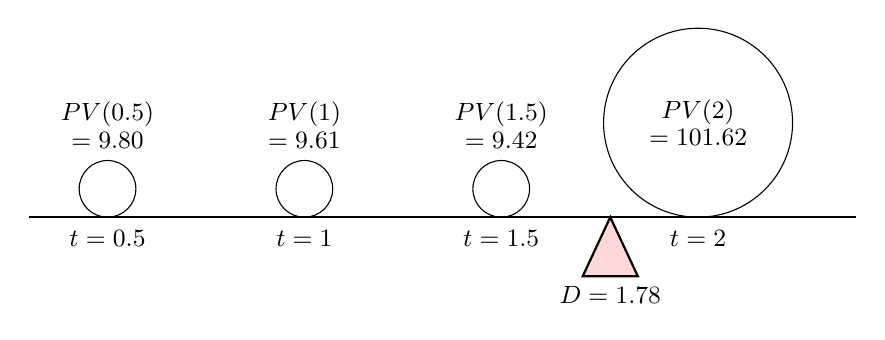
\begin{tikzpicture}[x=5cm]
        % beam
        \draw[thick] (0.3,0) -- (2.4,0);
        % weights: bigger PV = bigger circle
        \foreach \t/\pv in {0.5/9.80, 1/9.61, 1.5/9.42} {
            \draw (\t,0.36) circle (0.36cm);
            \node[above, align=center] at (\t,0.75) {\small $PV(\t)$\\[-2pt]\small $= \pv$};
            \node[below] at (\t,-0.05) {\small $t = \t$};
        }
        \draw (2,1.2) circle (1.2cm);
        \node[align=center] at (2,1.2) {\small $PV(2)$\\[-2pt]\small $= 101.62$};
        \node[below] at (2,-0.05) {\small $t = 2$};
        % fulcrum at the Macaulay duration
        \draw[thick, fill=red!15] (1.777,0) -- (1.707,-0.75) -- (1.847,-0.75) -- cycle;
        \node[below] at (1.777,-0.75) {\small $D = 1.78$};
    \end{tikzpicture}
    \end{center}
    Think of the PVs as weights on a seesaw over the timeline: the "balance point" is at $t = 1.78$, pulled close to $t = 2$ by the large final payment ($PV(2) = 101.62$). The formula above gives the same answer with $c = 0.2$, $\lambda = 0.04$, $m = 2$, $n = 4$.
    \\(Equivalently, the yield is $2\ln(1.02) = 3.9605\%$ continuously compounded.)
\end{example}

\heading{Modified Duration}
Why not calculate the sensitivity of a bond to the yield exactly?
\begin{definition}[\rb{Modified Duration}]
    Let $P$ be the price of a bond. The modified duration $D_m$ of the bond is
    \[\boxed{\begin{gathered}
        D_m = -\frac{1}{P(\lambda_0)}\left.\frac{dP(\lambda)}{d\lambda}\right|_{\lambda = \lambda_0}\\[4pt]
        \begin{aligned}
            \lambda_0 &: \text{the current yield}\\
            P(\lambda_0) &: \text{the current price of the bond}
        \end{aligned}
    \end{gathered}}\]
\end{definition}
\begin{itemize}
    \item Roughly, think \dbb{sensitivity = derivative}.
    \item The minus sign is so it won't be a negative quantity (price falls as yield rises).
    \item Dividing by $P$ makes it a \dbb{relative} sensitivity.
\end{itemize}

Modified duration gives the \ul{percentage change in price for a change in yield}:
\[D_m \approx -\frac{1}{P}\frac{\Delta P}{\Delta\lambda} \quad \Rightarrow \quad \boxed{\Delta P \approx -D_m P \Delta\lambda}\]

\begin{example}
    If the yield increases by 1\%, a bond with modified duration 5 drops in price by about 5\%.
    \\With a current price of \$100.
    \[\Delta P \approx -D_m P\Delta\lambda = -5(\$100)(0.01) = -\$5\]
\end{example}

\heading{Relationship between Modified and Macaulay Duration}
\[\boxed{\begin{gathered}
    D_m = \frac{D}{1+\frac{\lambda}{m}}\\[4pt]
    \begin{array}{@{}l@{}}
        D_m: \text{modified duration}\\
        D: \text{Macaulay duration}\\
        \lambda: \text{yield}\\
        m: \text{number of compounding periods per year}
    \end{array}
\end{gathered}}\]
\begin{enumerate}[label=(\roman*)]
    \item They differ only by a \dbb{constant factor}.
    \item With continuous compounding ($m\to\infty$), $D_m \to D$.
\end{enumerate}

\begin{proof}
    \b{Setup.} Suppose there are $m$ periods per year, the yield is $\lambda$, and the bond pays cash flow $c_k$ at period $k$ (time $k/m$ years), for $k = 0, 1, \dots, n$. Then
    \[PV_k = \frac{c_k}{\left(1+\frac{\lambda}{m}\right)^k}, \qquad \underset{\mathclap{\substack{\Big\uparrow\\\text{Current price of bond}}}}{PV_{tot}} = \sum_{k=0}^{n}PV_k = \sum_{k=0}^{n}\frac{c_k}{\left(1+\frac{\lambda}{m}\right)^k}\]
    and the two quantities we want to relate are
    \[D = \sum_{k=0}^{n}\frac{k}{m}\frac{PV_k}{PV_{tot}} \quad \text{(Macaulay)}, \qquad D_m = -\frac{1}{PV_{tot}}\frac{dPV_{tot}}{d\lambda} \quad \text{(modified)}\]

    \b{Step 1: differentiate the price.} Only $\left(1+\frac{\lambda}{m}\right)^{-k}$ depends on $\lambda$; by the chain rule,
    \[\frac{d}{d\lambda}\left(1+\frac{\lambda}{m}\right)^{-k} = -k\left(1+\frac{\lambda}{m}\right)^{-k-1}\cdot\frac{1}{m}\]
    so differentiating $PV_{tot}$ term by term gives
    \[\frac{dPV_{tot}}{d\lambda} = -\sum_{k=0}^{n}\frac{k}{m}\frac{c_k}{\left(1+\frac{\lambda}{m}\right)^{k+1}}\]

    \b{Step 2: rewrite in terms of $PV_k$.} Pull one factor of $\left(1+\frac{\lambda}{m}\right)$ out of each denominator:
    \[\frac{dPV_{tot}}{d\lambda} = -\frac{1}{1+\frac{\lambda}{m}}\sum_{k=0}^{n}\frac{k}{m}\underbrace{\frac{c_k}{\left(1+\frac{\lambda}{m}\right)^{k}}}_{PV_k} = -\frac{1}{1+\frac{\lambda}{m}}\sum_{k=0}^{n}\frac{k}{m}PV_k\]

    \b{Step 3: plug into the definition of $D_m$.}
    \begin{align*}
        D_m &= -\frac{1}{PV_{tot}}\frac{dPV_{tot}}{d\lambda}\\
        &= -\frac{1}{PV_{tot}}\left(-\frac{1}{1+\frac{\lambda}{m}}\sum_{k=0}^{n}\frac{k}{m}PV_k\right)\\
        &= \frac{1}{1+\frac{\lambda}{m}}\underbrace{\sum_{k=0}^{n}\frac{k}{m}\frac{PV_k}{PV_{tot}}}_{D}\\
        &= \frac{D}{1+\frac{\lambda}{m}}
    \end{align*}
\end{proof}
\rb{EXAM NOTE!} remember how to calculate the \rb{DERIVATIVE! } $\boxed{\left.\frac{dP(\lambda)}{d\lambda}\right|_{\lambda = \lambda_0}}$

\begin{example}
    A 10\%, 30-year bond priced at \$100 has Macaulay duration $D = 9.94$, with semi-annual coupons.
    \begin{enumerate}[label=(\alph*)]
        \item Modified duration, and the effect of a 1\% yield increase: since the price is \$100 (par), the yield is $\lambda = 10\%$, so
        \[D_m = \frac{D}{1+\frac{\lambda}{2}} = \frac{9.94}{1.05} = 9.47\]
        A 1\% increase in yield causes about a 9.47\% drop in price.
        \item Estimated price if the yield moves to 11\%:
        \[\Delta P \approx -D_m P\Delta\lambda = -9.47(100)(0.01) = -9.47 \quad \Rightarrow \quad P \approx \$100 - \$9.47 = \$90.53\]
    \end{enumerate}
\end{example}

\header{Duration with Spot Rates}
This time we compute sensitivity to changes in the \dbb{term structure} rather than the yield. It is again basically the derivative of the bond price with respect to interest rates, properly normalized, but now we \ul{perturb the entire spot rate curve}.

\heading{Sensitivity to Spot Rates}
Assume continuous compounding. What is the sensitivity of the present value of the cash flow $(x_{t_0}, x_{t_1}, \dots, x_{t_n})$ to \dbb{parallel shifts} in the spot rate curve?
\\Note that its assumed \underline{all spot rates change at the same rate}, hence parallel shift in the curve.

\begin{center}
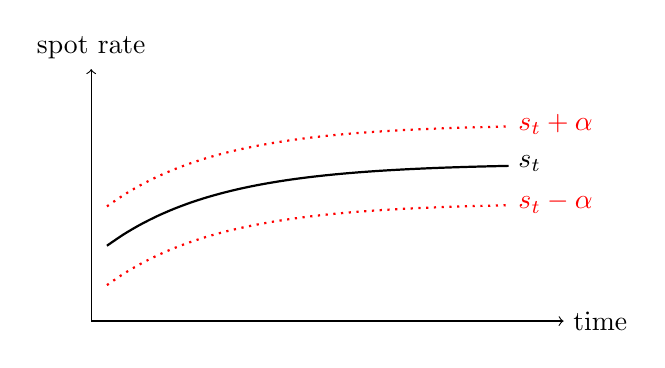
\begin{tikzpicture}
    \draw[->] (0,0) -- (6,0) node[right] {time};
    \draw[->] (0,0) -- (0,3.2) node[above] {spot rate};
    \draw[thick, domain=0.2:5.3, smooth, variable=\x] plot ({\x}, {2.0 - 1.2*exp(-0.7*\x)});
    \draw[thick, dotted, red, domain=0.2:5.3, smooth, variable=\x] plot ({\x}, {2.5 - 1.2*exp(-0.7*\x)});
    \draw[thick, dotted, red, domain=0.2:5.3, smooth, variable=\x] plot ({\x}, {1.5 - 1.2*exp(-0.7*\x)});
    \node[right] at (5.3,2.0) {$s_t$};
    \node[right, red] at (5.3,2.5) {$s_t + \alpha$};
    \node[right, red] at (5.3,1.5) {$s_t - \alpha$};
\end{tikzpicture}
\end{center}

Shift the whole curve by $\alpha$:
\[PV = \sum_{i=0}^{n}x_{t_i}e^{-s_{t_i}t_i} \quad \rightarrow \quad PV(\alpha) = \sum_{i=0}^{n}x_{t_i}e^{-(s_{t_i}+\alpha)t_i}\]
To determine sensitivity, \b{take the derivative with respect to $\alpha$ and evaluate at $\alpha = 0$}. Note that the current present value is $PV(0)$.

\begin{definition}[\rb{Duration with respect to Spot Rates}]
    \[\boxed{D(s_t) = \underset{\substack{\left\uparrow\vphantom{\rule{0pt}{6.5ex}}\right.\\\mathrlap{\hspace{-1.3cm}\text{price falls as rates rise } \left(\frac{dPV}{d\alpha} < 0\right)\text{,}}\\\mathrlap{\hspace{-1.3cm}\text{so the minus makes } D(s_t) > 0}}}{-}\Bigg(\underset{\mathclap{\substack{\Big\uparrow\\\text{current price}}}}{\frac{1}{PV(0)}}\Bigg)\underset{\mathclap{\substack{\Bigg\uparrow\\\text{shift curve by } \alpha}}}{\left.\frac{dPV(\alpha)}{d\alpha}\right|_{\alpha = 0}}}\]
    This is the \dbb{same recipe as modified duration}; only the thing we perturb changes:
    \[\underbrace{D_m = -\frac{1}{P(\lambda_0)}\left.\frac{dP(\lambda)}{d\lambda}\right|_{\lambda = \lambda_0}}_{\text{perturb the yield } \lambda} \qquad\longleftrightarrow\qquad \underbrace{D(s_t) = -\frac{1}{PV(0)}\left.\frac{dPV(\alpha)}{d\alpha}\right|_{\alpha = 0}}_{\text{perturb every spot rate by } \alpha}\]
    \begin{itemize}
        \item With \dbb{continuous compounding}, it is called the \rb{Fisher-Weil duration} (it looks similar to Macaulay!):
        \[\boxed{D_{FW} = \left(\frac{1}{PV}\right)\sum_{i=0}^{n}\underset{\mathclap{\substack{\Big\uparrow\\\text{time}}}}{t_i}\underbrace{x_{t_i}e^{-s_{t_i}t_i}}_{PV_{t_i}}}\]
        since $\left.\frac{dPV(\alpha)}{d\alpha}\right|_{\alpha=0} = -\sum_{i=0}^{n}t_i x_{t_i}e^{-s_{t_i}t_i}$.
        \\It is the same as the Macaulay duration, but generalized for all cash flow vectors, while Macaulay is for bonds.
        \\If the spot curve is flat ($s_{t_i} = \lambda$ for all $i$), then $D_{FW} = D$.
        \item With \dbb{discrete compounding} ($m$ periods per year, $s_i$ the spot rate for period $i$), it is called the \rb{quasi-modified duration}:
        \\Note it is not the Macaulay duration, as there is a factor of $+1$ in the power of the denominator.
        \\If the spot curve is flat ($s_i = \lambda$ for all $i$), then $D_Q = \frac{D}{1+\frac{\lambda}{m}} = D_m$.
    \end{itemize}
\end{definition}

\heading{Simplification for Continuous Compounding Only!}
Under continuous compounding, all the duration formulas look like a \dbb{weighted average of times}:
\[D_{FW} = \sum_{i=0}^{n}t_i\frac{PV_{t_i}}{PV_{Total}}\]
The only difference is the rate used to compute the PVs:
\begin{itemize}
    \item Macaulay and modified duration use the \dbb{yield}: $PV_{t_i} = x_{t_i}e^{-\lambda t_i}$
    \item Fisher-Weil duration uses the \dbb{spot rates}: $PV_{t_i} = x_{t_i}e^{-s_{t_i}t_i}$
\end{itemize}

\begin{example}
    \begin{center}
    \begin{tikzpicture}
        \draw[->] (0,0) -- (6,0) node[right] {time};
        \draw[->] (0,0) -- (0,2.8) node[above] {spot rate};
        \draw[thick, domain=0.2:5.3, smooth, variable=\x] plot ({\x}, {2.2 - 1.2*exp(-0.7*\x)});
        \draw[thick, dotted, red, domain=0.2:5.3, smooth, variable=\x] plot ({\x}, {1.7 - 1.2*exp(-0.7*\x)});
        \node[right] at (5.3,2.2) {$s_t$};
        \node[right, red] at (5.3,1.7) {$s_t - 2\%$};
    \end{tikzpicture}
    \end{center}
    The entire spot rate curve drops by 2\%. A bond with Fisher-Weil duration 10 changes in price by approximately $-D_{FW}\Delta\alpha = -10(-0.02) = +20\%$, i.e.\ it \dbb{increases by 20\%}.
\end{example}

\header{Summary}
\begin{framed}
    \b{Macaulay duration} is a weighted average of the times to cash flows:
    \[D = w_{t_1}t_1 + w_{t_2}t_2 + \cdots + w_{t_n}t_n, \qquad w_{t_i} = \frac{PV(t_i)}{PV_{total}}\]
    The other durations measure a percentage change in price for a change in either the yield or a parallel shift of the spot rate curve.
    \begin{itemize}
        \item \b{Modified duration} uses the yield, and is related to Macaulay duration by
        \[D_m = -\frac{1}{P(\lambda_0)}\left.\frac{dP(\lambda)}{d\lambda}\right|_{\lambda=\lambda_0}, \qquad D_m = \frac{D}{1+\frac{\lambda}{m}}\]
        \item \b{Fisher-Weil} (continuous compounding) and \b{quasi-modified} (discrete compounding) use the spot rate curve:
        \[D(s_t) = -\left(\frac{1}{PV(0)}\right)\left.\frac{dPV(\alpha)}{d\alpha}\right|_{\alpha=0}\]
        \[D_{FW} = \left(\frac{1}{PV}\right)\sum_{i=0}^{n}t_i x_{t_i}e^{-s_{t_i}t_i}, \qquad D_Q = \left(\frac{1}{PV}\right)\sum_{i=1}^{n}\frac{\frac{i}{m}x_i}{\left(1+\frac{s_i}{m}\right)^{i+1}}\]
    \end{itemize}
\end{framed}

% !TeX root = ../main.tex

\newlecture[Duration for Bond Portfolios \& Immunization][Oct 8, 2026]

\header{Duration of a Portfolio}
\begin{definition}[\rb{Portfolio Duration}]
    Given fixed income securities with prices $P_i$ and durations $D_i$, $i = 1, \dots, m$, the portfolio consisting of the aggregate of these has price $P$ and duration $D$:
    \[\boxed{\begin{gathered}
        P = P_1 + P_2 + \cdots + P_m\\
        D = w_1D_1 + w_2D_2 + \cdots + w_mD_m, \qquad w_i = \frac{P_i}{P}
    \end{gathered}}\]
    Works for both \dbb{Macaulay} and \dbb{all forms of modified} duration.
\end{definition}
\keypoint{\db{Note}: this looks just like the Macaulay duration formula, except with \rb{time replaced by duration}!\\(Weights are each security's share of the total price.)}

\heading{Derivation}
Take two cash flow streams $A$ and $B$ over the same times $t_0, \dots, t_n$ (a stream with no payment at $t_k$ just has $PV_k = 0$ there):
\begin{center}
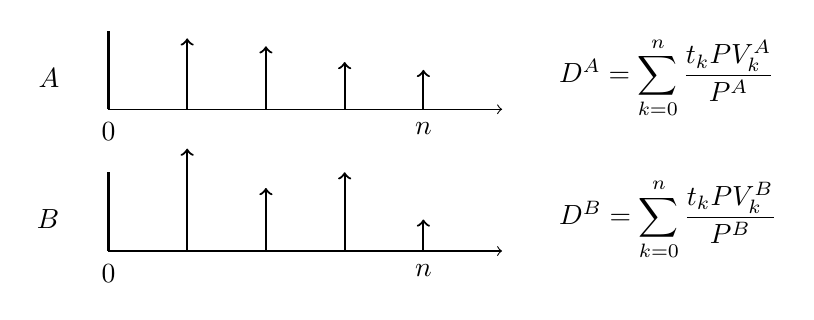
\begin{tikzpicture}
    \foreach \row/\lab/\hs in {0/A/{0.9,0.8,0.6,0.5}, -1.8/B/{1.3,0.8,1.0,0.4}} {
        \begin{scope}[yshift=\row cm]
            \node[left] at (-0.5,0.4) {$\lab$};
            \draw[->] (0,0) -- (5,0);
            \draw[thick] (0,0) -- (0,1.0);
            \node[below] at (0,-0.05) {$0$};
            \node[below] at (4,-0.05) {$n$};
            \foreach \h [count=\k] in \hs { \draw[->, thick] (\k,0) -- (\k,\h); }
            \node[right] at (5.6,0.4) {$D^{\lab} = \displaystyle\sum_{k=0}^{n}\frac{t_k PV_k^{\lab}}{P^{\lab}}$};
        \end{scope}
    }
\end{tikzpicture}
\end{center}
The duration of $A + B$ (cash flows add, so PVs add):
\begin{align*}
    D^{A+B} &= \sum_{k=0}^{n}\frac{t_k\left(PV_k^A + PV_k^B\right)}{P^A + P^B}
    = \sum_{k=0}^{n}\frac{t_kPV_k^A}{P^A + P^B} + \sum_{k=0}^{n}\frac{t_kPV_k^B}{P^A + P^B}\\
    &= \sum_{k=0}^{n}\frac{t_kPV_k^A}{P^A + P^B}\cdot\textcolor{red!70!black}{\frac{P^A}{P^A}} + \sum_{k=0}^{n}\frac{t_kPV_k^B}{P^A + P^B}\cdot\textcolor{red!70!black}{\frac{P^B}{P^B}} && \text{(multiply by 1)}\\
    &= \underbrace{\sum_{k=0}^{n}\frac{t_kPV_k^A}{\textcolor{red!70!black}{P^A}}}_{D^A}\left(\frac{\textcolor{red!70!black}{P^A}}{P^A + P^B}\right) + \underbrace{\sum_{k=0}^{n}\frac{t_kPV_k^B}{\textcolor{red!70!black}{P^B}}}_{D^B}\left(\frac{\textcolor{red!70!black}{P^B}}{P^A + P^B}\right) && \text{(swap denominators)}
\end{align*}
\[\boxed{D^{A+B} = \left(\frac{P^A}{P^A + P^B}\right)D^A + \left(\frac{P^B}{P^A + P^B}\right)D^B = w_AD^A + w_BD^B}\]
The weights add to 1 ($w_A + w_B = 1$), so $D^{A+B}$ always lies \ul{between} $D^A$ and $D^B$ (for positive prices). Repeating this for more streams gives the general formula.
\\Note: the derivation needs every $PV_k$ to be computed with the \ul{same rate} (one common yield, or one spot rate curve). If the bonds have different yields, the formula is only an approximation.

\header{Immunization}
\begin{definition}[\rb{Immunization}]
    Constructing a portfolio of bonds which is \dbb{protected (immunized) against changes in interest rates}.
\end{definition}

\b{Problem}: you have an obligation to pay \$1,000 two years from now, but you can only purchase bonds of maturity 1 and 5 years.
\begin{itemize}
    \item 1 year bond only: \dbb{reinvestment risk}. The money must be reinvested at year 1 at an unknown future rate.
    \item 5 year bond only: \dbb{too sensitive to interest rates}. It must be sold at year 2 at an unknown price.
\end{itemize}

\begin{center}
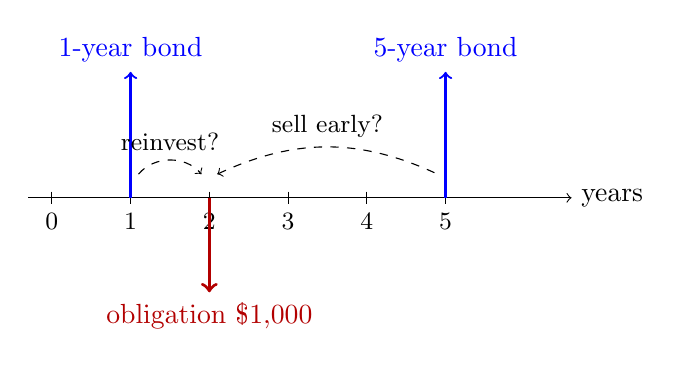
\begin{tikzpicture}
    \draw[->] (-0.3,0) -- (6.6,0) node[right] {years};
    \foreach \x in {0,...,5} { \draw (\x,0.08) -- (\x,-0.08) node[below] {\small \x}; }
    \draw[->, very thick, red!70!black] (2,0) -- (2,-1.2) node[below] {obligation \$1,000};
    \draw[->, thick, blue] (1,0) -- (1,1.6) node[above] {1-year bond};
    \draw[->, thick, blue] (5,0) -- (5,1.6) node[above] {5-year bond};
    \draw[->, dashed] (1.1,0.3) to[bend left=50] node[above] {\small reinvest?} (1.9,0.3);
    \draw[<-, dashed] (2.1,0.3) to[bend left=25] node[above] {\small sell early?} (4.9,0.3);
\end{tikzpicture}
\end{center}

\keypoint{\rb{Solution}: construct a portfolio of 1 and 5 year securities with the same \rb{present value} and \rb{duration} as your obligation.}

With $x$ units of bond 1 (price $P_1$, duration $D_1$) and $y$ units of bond 2 (price $P_2$, duration $D_2$), and an obligation with present value $P$ and duration $D$:
\[\boxed{\begin{aligned}
    \text{PV:} &\quad xP_1 + yP_2 = P\\
    \text{Duration:} &\quad \frac{xP_1}{P}D_1 + \frac{yP_2}{P}D_2 = D
\end{aligned}}\]
Solve these two equations for $x$ and $y$ to determine your portfolio. The duration equation is just the portfolio duration formula, with weights $w_1 = \frac{xP_1}{P}$ and $w_2 = \frac{yP_2}{P}$.

\b{Why it works}: equal PV means equal value \ul{now}. Equal duration means equal $\frac{dP}{d\lambda}$ (since $\frac{dP}{d\lambda} = -D_mP$), so when the yield moves a little, the portfolio and the obligation \ul{change in value by about the same amount}. The portfolio can still cover the obligation.

\begin{example}
    You have an obligation of \$1,000 in 2 years, and wish to invest now to meet it. You can invest in 1 year and 5 year zero-coupon bonds (face \$100, discrete yearly compounding, yield 9\%):
    \begin{center}
    \begin{tabular}{lccccc}
        \toprule
        & Coupon & Maturity & Yield & Price & Duration (Mac)\\
        \midrule
        \textcolor{red!70!black}{Obligation} & \multicolumn{3}{c}{\textcolor{red!70!black}{\$1,000 in 2 years}} & \textcolor{red!70!black}{\$841.68} & \textcolor{red!70!black}{2 years}\\
        \db{Bond 1} & 0\% & 1 year & 9\% & \$91.74 & 1 year\\
        \db{Bond 2} & 0\% & 5 years & 9\% & \$64.99 & 5 years\\
        \bottomrule
    \end{tabular}
    \end{center}
    Prices: $\frac{1000}{1.09^2} = 841.68$, $\frac{100}{1.09} = 91.74$, $\frac{100}{1.09^5} = 64.99$. Each is a zero, so its Macaulay duration is its maturity.
    \\Let $x$ = number of bond 1, $y$ = number of bond 2 held.
    \begin{align*}
        \text{Match prices:} &\quad 91.74x + 64.99y = 841.68\\
        \text{Match durations:} &\quad \frac{91.74x}{841.68}(1\text{ year}) + \frac{64.99y}{841.68}(5\text{ years}) = 2\text{ years}
    \end{align*}
    Multiplying the duration equation by 841.68 and subtracting the price equation: $4(64.99)y = 841.68$, so
    \[\boxed{x = 6.88, \quad y = 3.24}\]
    In weights, $w_1 + w_2 = 1$ and $w_1(1) + w_2(5) = 2$ give $w_1 = \frac{3}{4}$ and $w_2 = \frac{1}{4}$. So \$631.26 goes into bond 1 and \$210.42 into bond 2.
\end{example}

\begin{example}[Bond Immunization Spreadsheet]
    Yield 9\% (semi-annual compounding, 4.5\% per period). Obligation of \$1,000,000 in 10 years, to be immunized using:
    \begin{center}
    \begin{tabular}{lcccccc}
        \toprule
        & Maturity & Principal & Coupon & Price & Macaulay $D$ & \$ amount\\
        \midrule
        Bond 1 & 20 & \$1,000 & 4\% & \$539.96 & 11.45191 & \$321,333.61\\
        Bond 2 & 5 & \$1,000 & 0\% & \$643.93 & 5 & \$93,309.25\\
        \midrule
        Obligation & 10 & \$1,000,000 & 0\% & \$414,642.86 & 10 & \$414,642.86\\
        \bottomrule
    \end{tabular}
    \end{center}
    \begin{itemize}
        \item Prices at 4.5\% per period, e.g.\ bond 2: $\frac{1000}{1.045^{10}} = 643.93$, obligation: $\frac{1{,}000{,}000}{1.045^{20}} = 414{,}642.86$.
        \item Match durations with weights: $11.45191\,w_1 + 5(1 - w_1) = 10 \;\Rightarrow\; w_1 = \frac{5}{6.45191} = 0.775$.
        \item \$ amounts: $0.775(414{,}642.86) = \$321{,}333.61$ in bond 1, and the rest, \$93,309.25, in bond 2.
        \item Number of bonds $= \frac{\$\text{ amount}}{\text{price}}$: \dbb{595.1059} of bond 1 and \dbb{144.9064} of bond 2.
    \end{itemize}
    Note the target duration (10) must lie \ul{between} the two bonds' durations (5 and 11.45). Otherwise one weight is negative, i.e.\ a short position.
\end{example}

\header{The Real Idea Behind Immunization: Taylor Expansions!}
With $\lambda_0$ the current value of the yield, expand the price as a function of the yield around the current value:
\[\boxed{P(\lambda) = \underset{\mathclap{\substack{\Big\uparrow\\\text{price}}}}{P(\lambda_0)} + \underbrace{P'(\lambda_0)(\lambda - \lambda_0)}_{\text{duration}} + \underbrace{\tfrac{1}{2}P''(\lambda_0)(\lambda - \lambda_0)^2}_{\text{convexity}} + \cdots}\]
Here duration and convexity are \dbb{unnormalized}: $P'(\lambda_0) = -D_mP(\lambda_0)$ is modified duration times price.

\keypoint{You can match as many terms as you like to make the Taylor series of your portfolio look like the Taylor series of your cash flow stream (obligation).}

\begin{itemize}
    \item Matching \b{PV and duration} (as above) matches the first two terms. The portfolio and obligation price-yield curves are \dbb{tangent} at $\lambda_0$.
    \item Matching \b{convexity} too would match the curvature, but needs a third equation, so a third bond.
\end{itemize}

\begin{center}
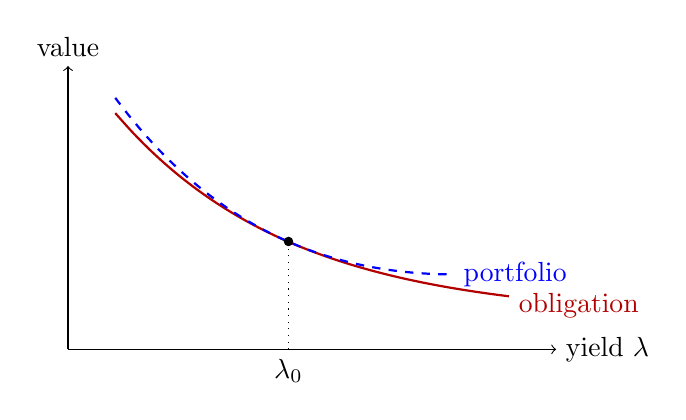
\begin{tikzpicture}
    \draw[->] (0,0) -- (6.2,0) node[right] {yield $\lambda$};
    \draw[->] (0,0) -- (0,3.6) node[above] {value};
    \draw[thick, red!70!black, domain=0.6:5.6, smooth, variable=\x] plot ({\x}, {0.4 + 2.6*exp(-0.45*(\x-0.6))});
    \draw[thick, blue, dashed, domain=0.6:4.9, smooth, variable=\x] plot ({\x}, {0.4 + 2.6*exp(-0.45*(\x-0.6)) + 0.04*(\x-2.8)^2});
    \draw[dotted] (2.8,0) -- (2.8,1.37);
    \node[below] at (2.8,0) {$\lambda_0$};
    \filldraw (2.8,1.37) circle (1.5pt);
    \node[red!70!black, right] at (5.6,0.55) {obligation};
    \node[blue, right] at (4.9,0.95) {portfolio};
\end{tikzpicture}
\end{center}
Same value and slope at $\lambda_0$, so small yield changes affect both equally. For larger changes, the curvature (convexity) difference shows up.


\end{document}
